\chapter{Eredmények}
\label{ch:results}

\section{Vizsgált kódbázisok}

Egy kódbázisnak a következő feltételeket kell teljesíteni, hogy vizsgálni tudjuk:
\begin{enumerate}
    \item Legyen könnyen build-elhető, évekre visszamenően
    \item A tesztek legyenek könnyen futtathatóak
    \item Generálódjon coverage report a teszt futtatásokhoz és a report formátuma legyen egyike azoknak, amiket támogat a ReportGenerator\footnote{https://github.com/danielpalme/ReportGenerator} nevű .NET-es könyvtár
    \item A projekt legyen nyílt forráskódú
    \item Rendelkezzen a projekt viszonylag gazdag commit történettel -- jelen esetben az 5000+ commit és 3+ éves történet heurisztikát alkalmaztam
\end{enumerate}

Ezeket a feltételeket ugyan könnyű teljesíteni egy fejlesztő csapatnak ipari környezetben saját projektekre, sajnos nyílt forráskódú környezetben más a helyzet -- specifikusan az 1-es és 3-as pontok jelentenek problémát. A C++-ra, Python-ra és .NET Framework-re épülő projektek például egy az egyben kiesnek, mert egyik sem ad egyszerű módot arra, hogy a build-eléshez szükséges környezetet könnyen elő tudjuk állítani a projekt életciklusának akármely pontján.

Gyakorlatban a JavaScript NodeJS/NPM, .NET Core/.NET 5+ és Java ökoszisztémákra épülő projektek felelhetnek meg a korábbi feltételeknek. Ezek közül azonban a Java a szakmai hátterem miatt kiesik, a .NET Core/5+ projektek jelentős többsége pedig az 5-ös feltételt nem teljesíteni, így marad a JavaScript Node/NPM ökoszisztéma. A specifikus projekteknél külön meg fogom említeni, de általánosságban itt is leírom: még a JavaScript/NodeJS/NPM ökoszisztéma esetén is komoly problémát jelent a régi (~2015 előtti) verziók build-elése, mivel az NPM és a node, illetve a rájuk épített projektek sok változáson estek át az évek során, amit ma a projekt ismerete nélkül már nehéz reprodukálni. Ez azt jelenti, hogy a legtöbb esetben lehetetlen

Fontos leszögezni még egy dolgot. A JavaScript-es projektek elemzése egy jelentős vakfoltot fog képezni, méghozzá azért, mert a nyílt forráskódú projektek között gyakorlatilag lehetetlen olyat találni, amire őszintén azt lehet mondani, hogy rossz minőségű kódbázissal rendelkezik. Nyilván egy kódbázis minősége szubjektív, de a GitHub-on host-olt JavaScript projektek túlnyomó többsége 95\% feletti coverage-el rendelkezik. Ráadásul azok a projektek, amik 95\% alatt vannak, azok jellemzően csak a nagyon konzervatív coverage ignore path-ok miatt mutatnak ilyen értékeket -- a React projekt például 80\% körüli értéket mutatott, azonban hamar kiderült, hogy ez csak azért van, mert halott kódot tartanak a repository-ban, amit már nem hajtanak meg unit tesztek.

A fentieket figyelembe véve a következő projektekre esett a választás:
\begin{itemize}
    \item Vue: https://github.com/vuejs/vue
    \item Express: https://github.com/expressjs/express
    \item React: https://github.com/facebook/react
    \item Gatsby: https://github.com/gatsbyjs/gatsby
\end{itemize}

\section{Vue}

Elsőként a vue.js\footnote{https://github.com/vuejs/vue} kódbázisát fogjuk megvizsgálni. A Vue egy progresszív, JavaScript-alapú frontend framework. A Vue feature-ök tekintetében valahol a később taglalt Angular és React között van -- nem próbál egy kikövezett utat adni, mint az Angular, de nem csak egy specifikus szeletét fedi le a frontend fejlesztésnek, mint a React.

\lstset{language=HTML, caption={Egy egyszerű Vue komponens}}
\begin{lstlisting}
<div id="app">
    {{ message }}
</div>
\end{lstlisting}

\lstset{language=JavaScript, caption={Egy egyszerű Vue komponens}}
\begin{lstlisting}
var app = new Vue({
    el: '#app',
    data: {
        message: 'Hello Vue!'
    }
})
\end{lstlisting}

A projekt viszonylag fiatal, fejlesztése 2016-ban kezdődött. A későbbi megfigyelések szempontjából fontos megjegyezni, hogy ugyan jelen pillanatban 338 egyedi kontribútora van a projektnek, a fejlesztés nagy része egy fejlesztőhöz, Evan You nevéhez köthető:

\lstset{caption={A vue.js top 10 kontribútora}}
\begin{lstlisting}
vue git:(dev) git shortlog -sn | head -n10
    2303  Evan You
    78  vue-bot
    47  Hanks
    34  Eduardo San Martin Morote
    32  kazuya kawaguchi
    30  chengchao
    25  katashin
    21  AchillesJ
    18  Herrington Darkholme
    15  JK
\end{lstlisting}

Az analízist a vue esetében az első publikus release-től kezdjük.
\pagebreak

\subsection{Vue 1.0}

A vue több szempontból is különös eset lesz: egyrészt az első publikus release-ig gyakorlatilag egy egyszemélyes projekt volt, másrészt pedig, ahogy azt később látni fogjuk, a Vue 2.0 egy teljes újraírása volt a projektnek.

Először vessünk egy pillantást a \ref{table:vue1-top-files} táblázatra, amiben a vue 1.0-ás változatának legtöbbet módosított fájljai láthatóak. Látható, hogy bár egy fejlesztője van a projektnek és 100\%-os coverage-el rendelkezik, már itt kialakulóban van fájloknak egy halmaza, amik vonzani fogják magukhoz a későbbi változtatásokat és javításokat. A \code{compile.js}, \code{directive.js} és \code{watcher.js} fájlokra kiemelten érdemes figyelni, mert ezek már most kiemelkednek az átlagból méret és változtatások száma tekintetében (átlag fájl méret 147, átlag változtatások száma 20 a teljes repository-ra).

\begin{table}[h]
    \centering
    \begin{tabular}{l|l|l|l|l}
        Filename      & Lifetime Authors & Lifetime Changes & Line Count & Coverage \% \\ \hline
        compile.js    & 2                & 123              & 709        & 100         \\
        directive.js  & 1                & 102              & 320        & 100         \\
        init.js       & 1                & 80               & 114        & 100         \\
        watcher.js    & 3                & 72               & 344        & 100         \\
        vue.js        & 1                & 52               & 96         & 100         \\
        lifecycle.js  & 1                & 49               & 68         & 100         \\
        data.js       & 1                & 45               & 174        & 100         \\
        lang.js       & 4                & 44               & 388        & 100         \\
        dom.js        & 2                & 42               & 362        & 100         \\
        transclude.js & 2                & 40               & 148        & 100         \\
        global.js     & 1                & 39               & 152        & 100
    \end{tabular}
    \caption{A vue 1.0-ás kiadásának leggyakrabban módosított fájljai} \label{table:vue1-top-files}
\end{table}

\begin{figure}[H]
    \centering
    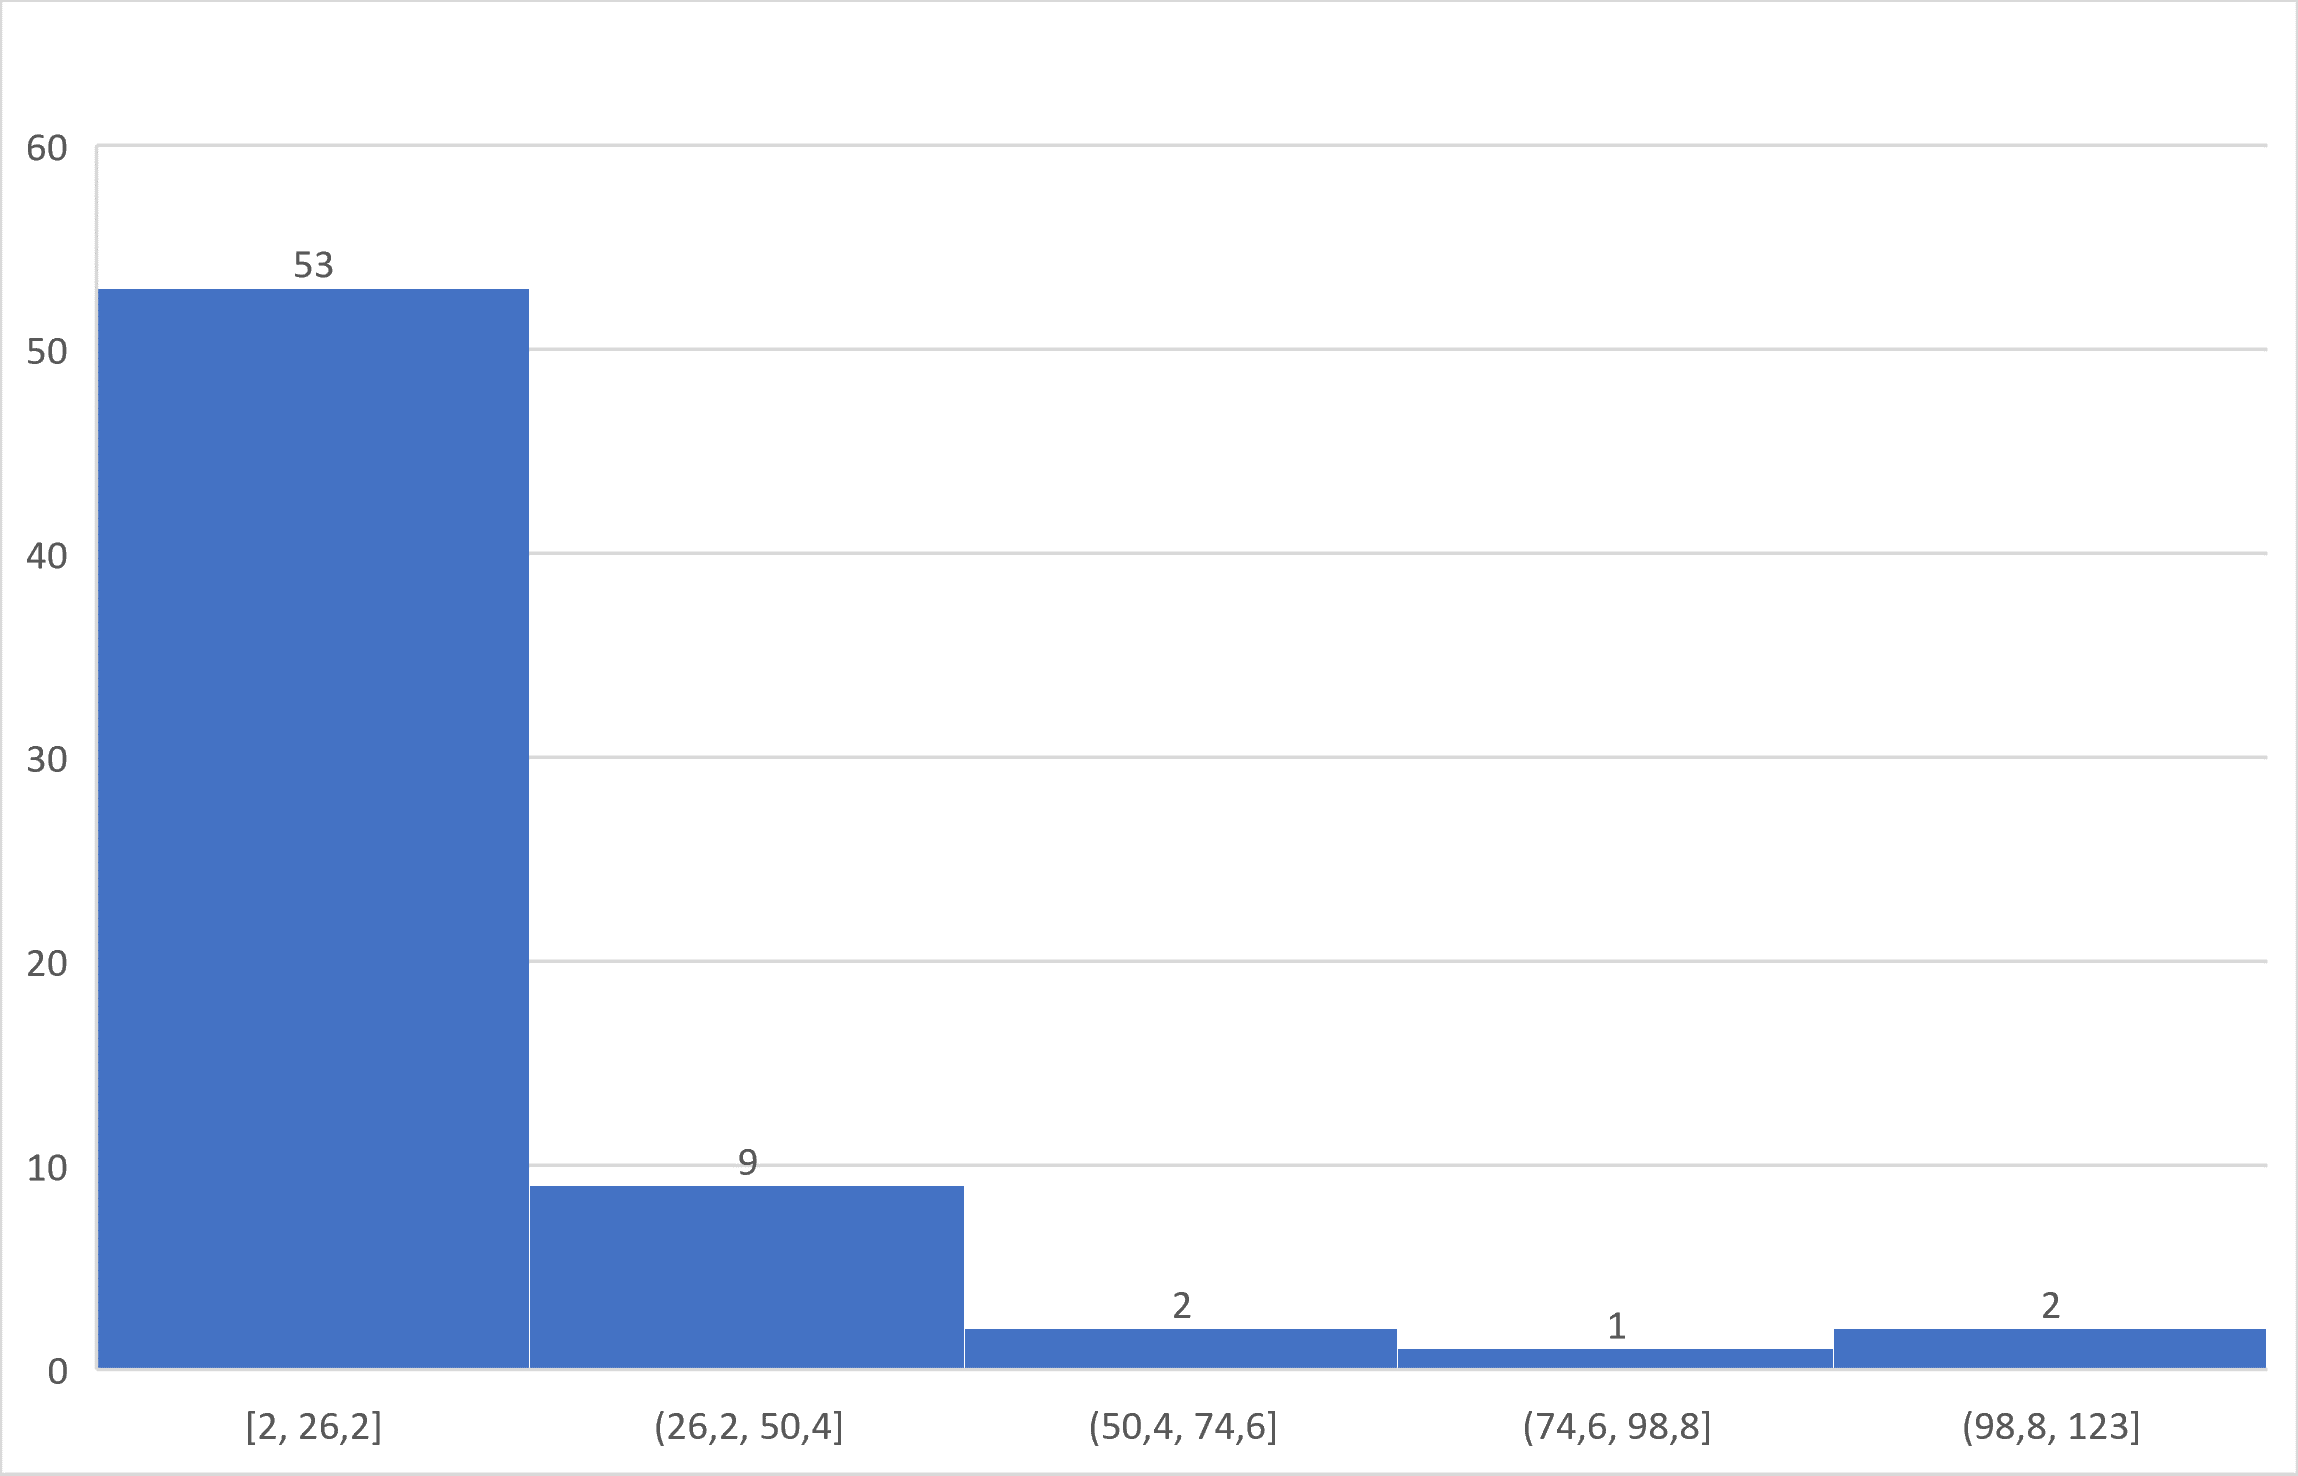
\includegraphics[width=1\textwidth]{images/vue/vue1-hist.png}
    \caption{Fájlonkénti változtatások számának a hisztogramja}
    \label{fig:vue1-hist}
\end{figure}

Érdekes továbbá a változtatások számáról készített hisztogram a \ref{fig:vue1-hist} ábrán, amiről jól látszik, hogy a 67 forrás fájlból álló vue 1.0 változtatásainak egy jelentős része 5 fájl köré csoportosul, amik méret és változtatás szám szepontjából már most az átlag többszörösét mutatják.



\begin{figure}[H]
    \centering
    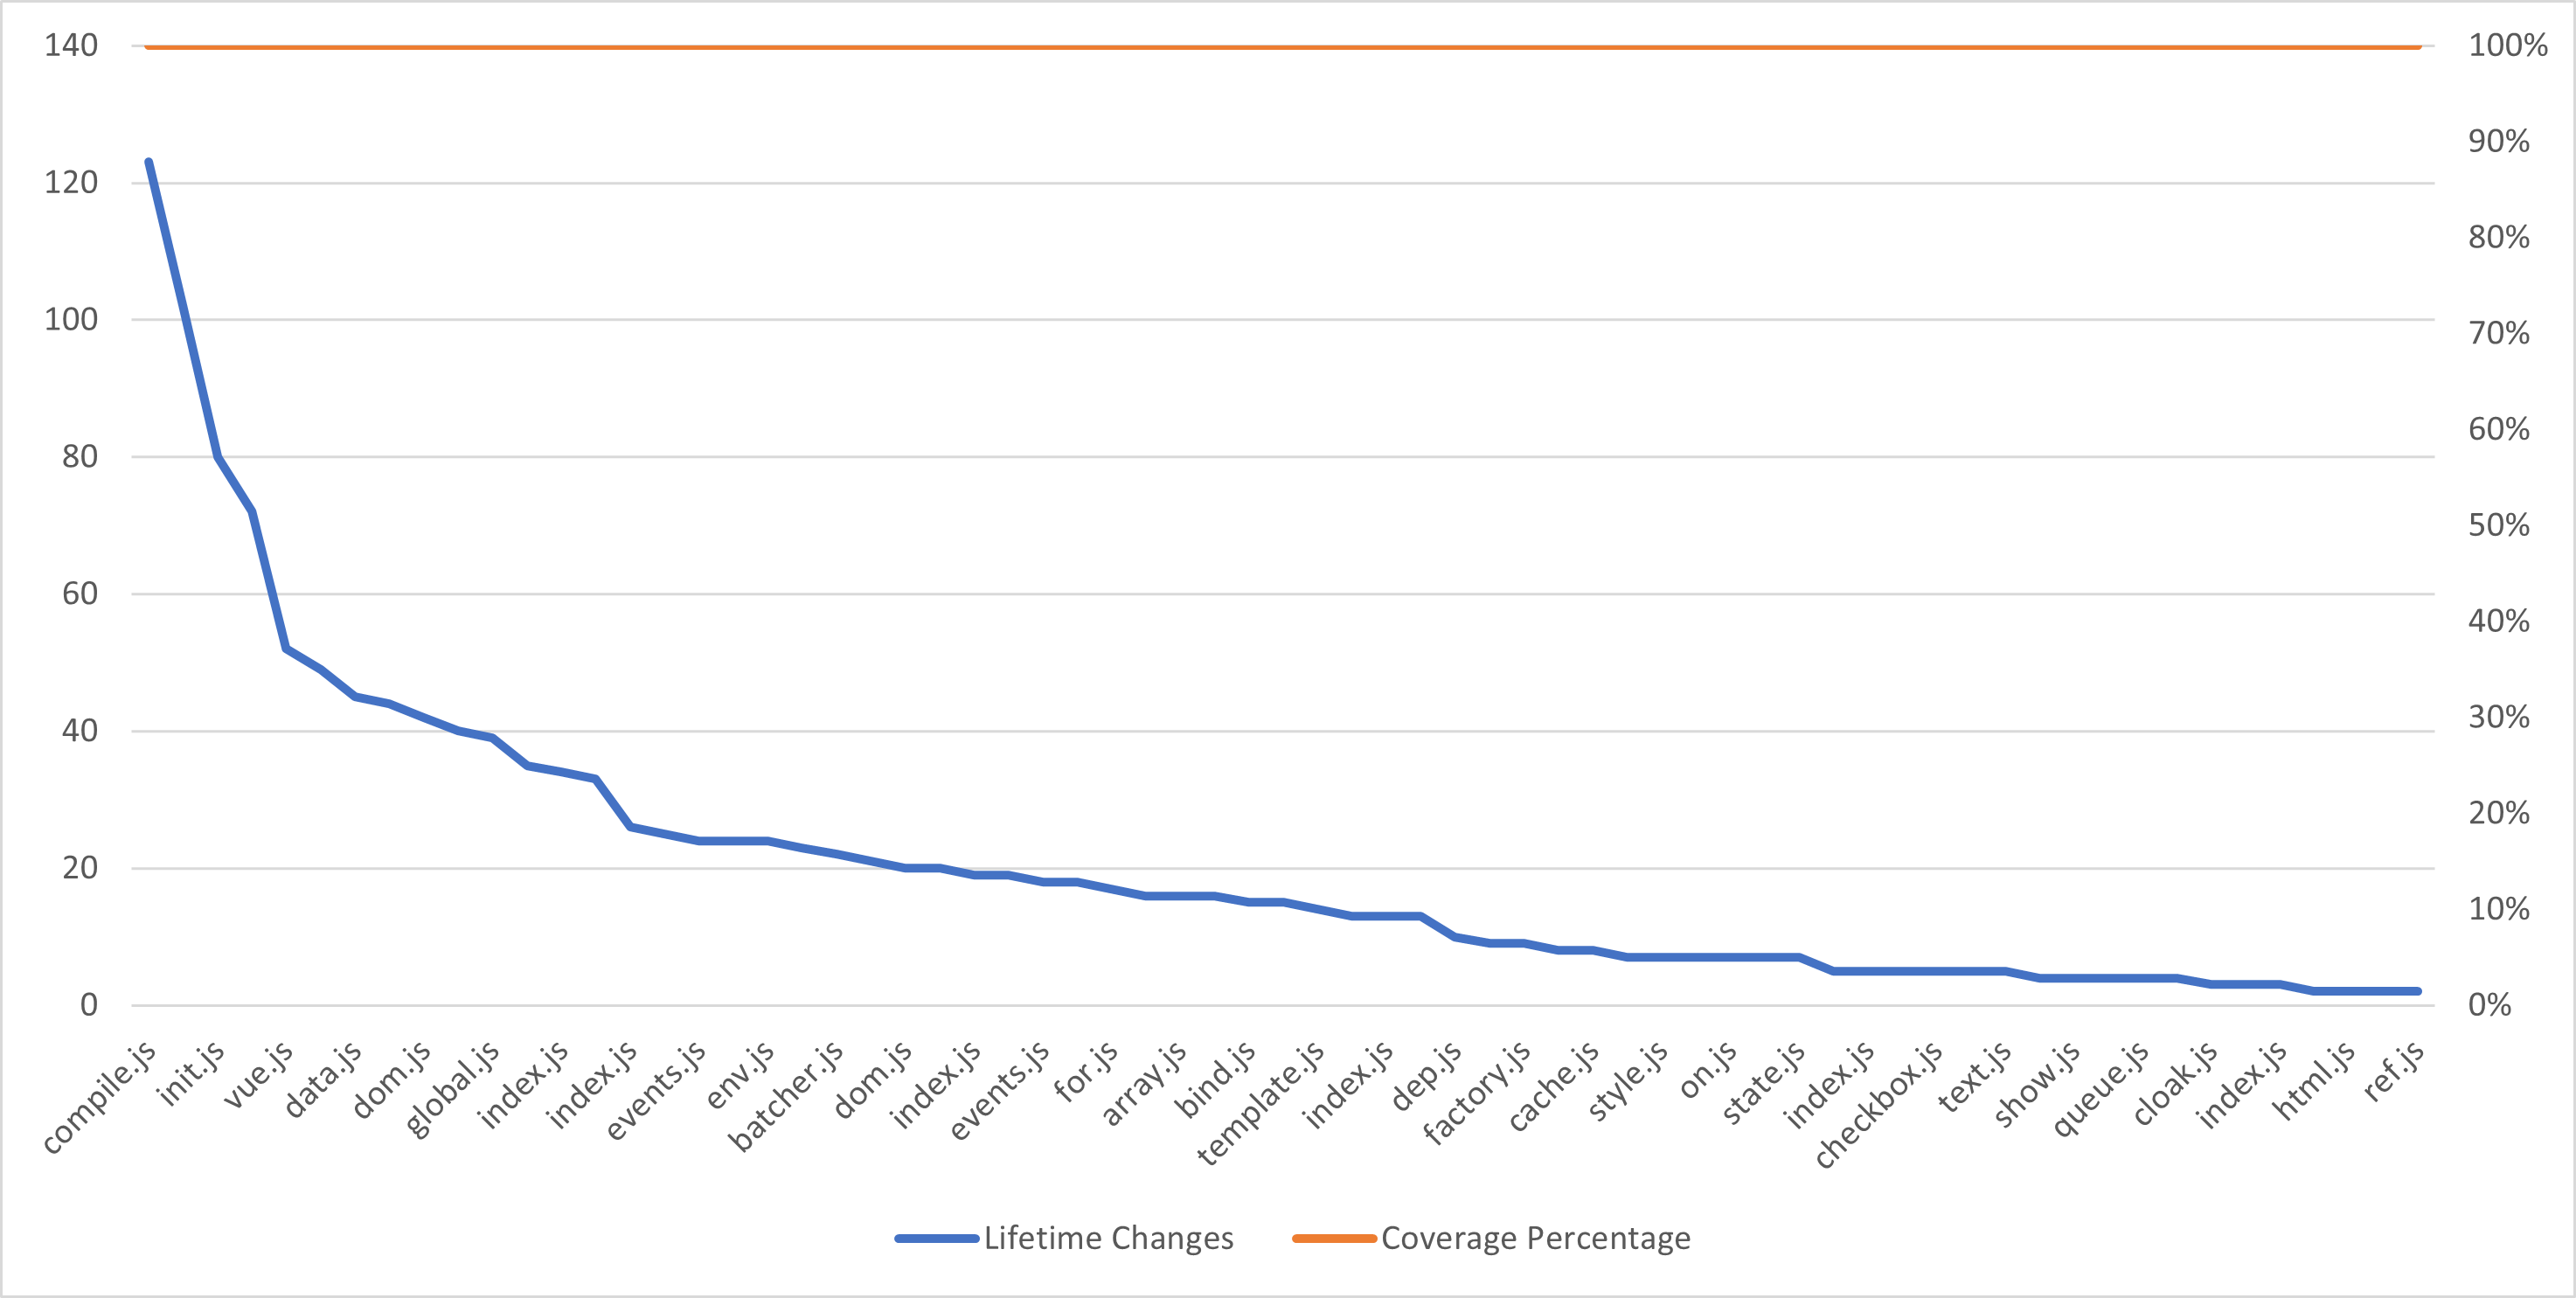
\includegraphics[width=1\textwidth]{images/vue/vue1-lifetime-changes.png}
    \caption{A vékony kliens által generált grafikonok}
    \label{fig:hestia-charts}
\end{figure}

\begin{figure}[H]
    \centering
    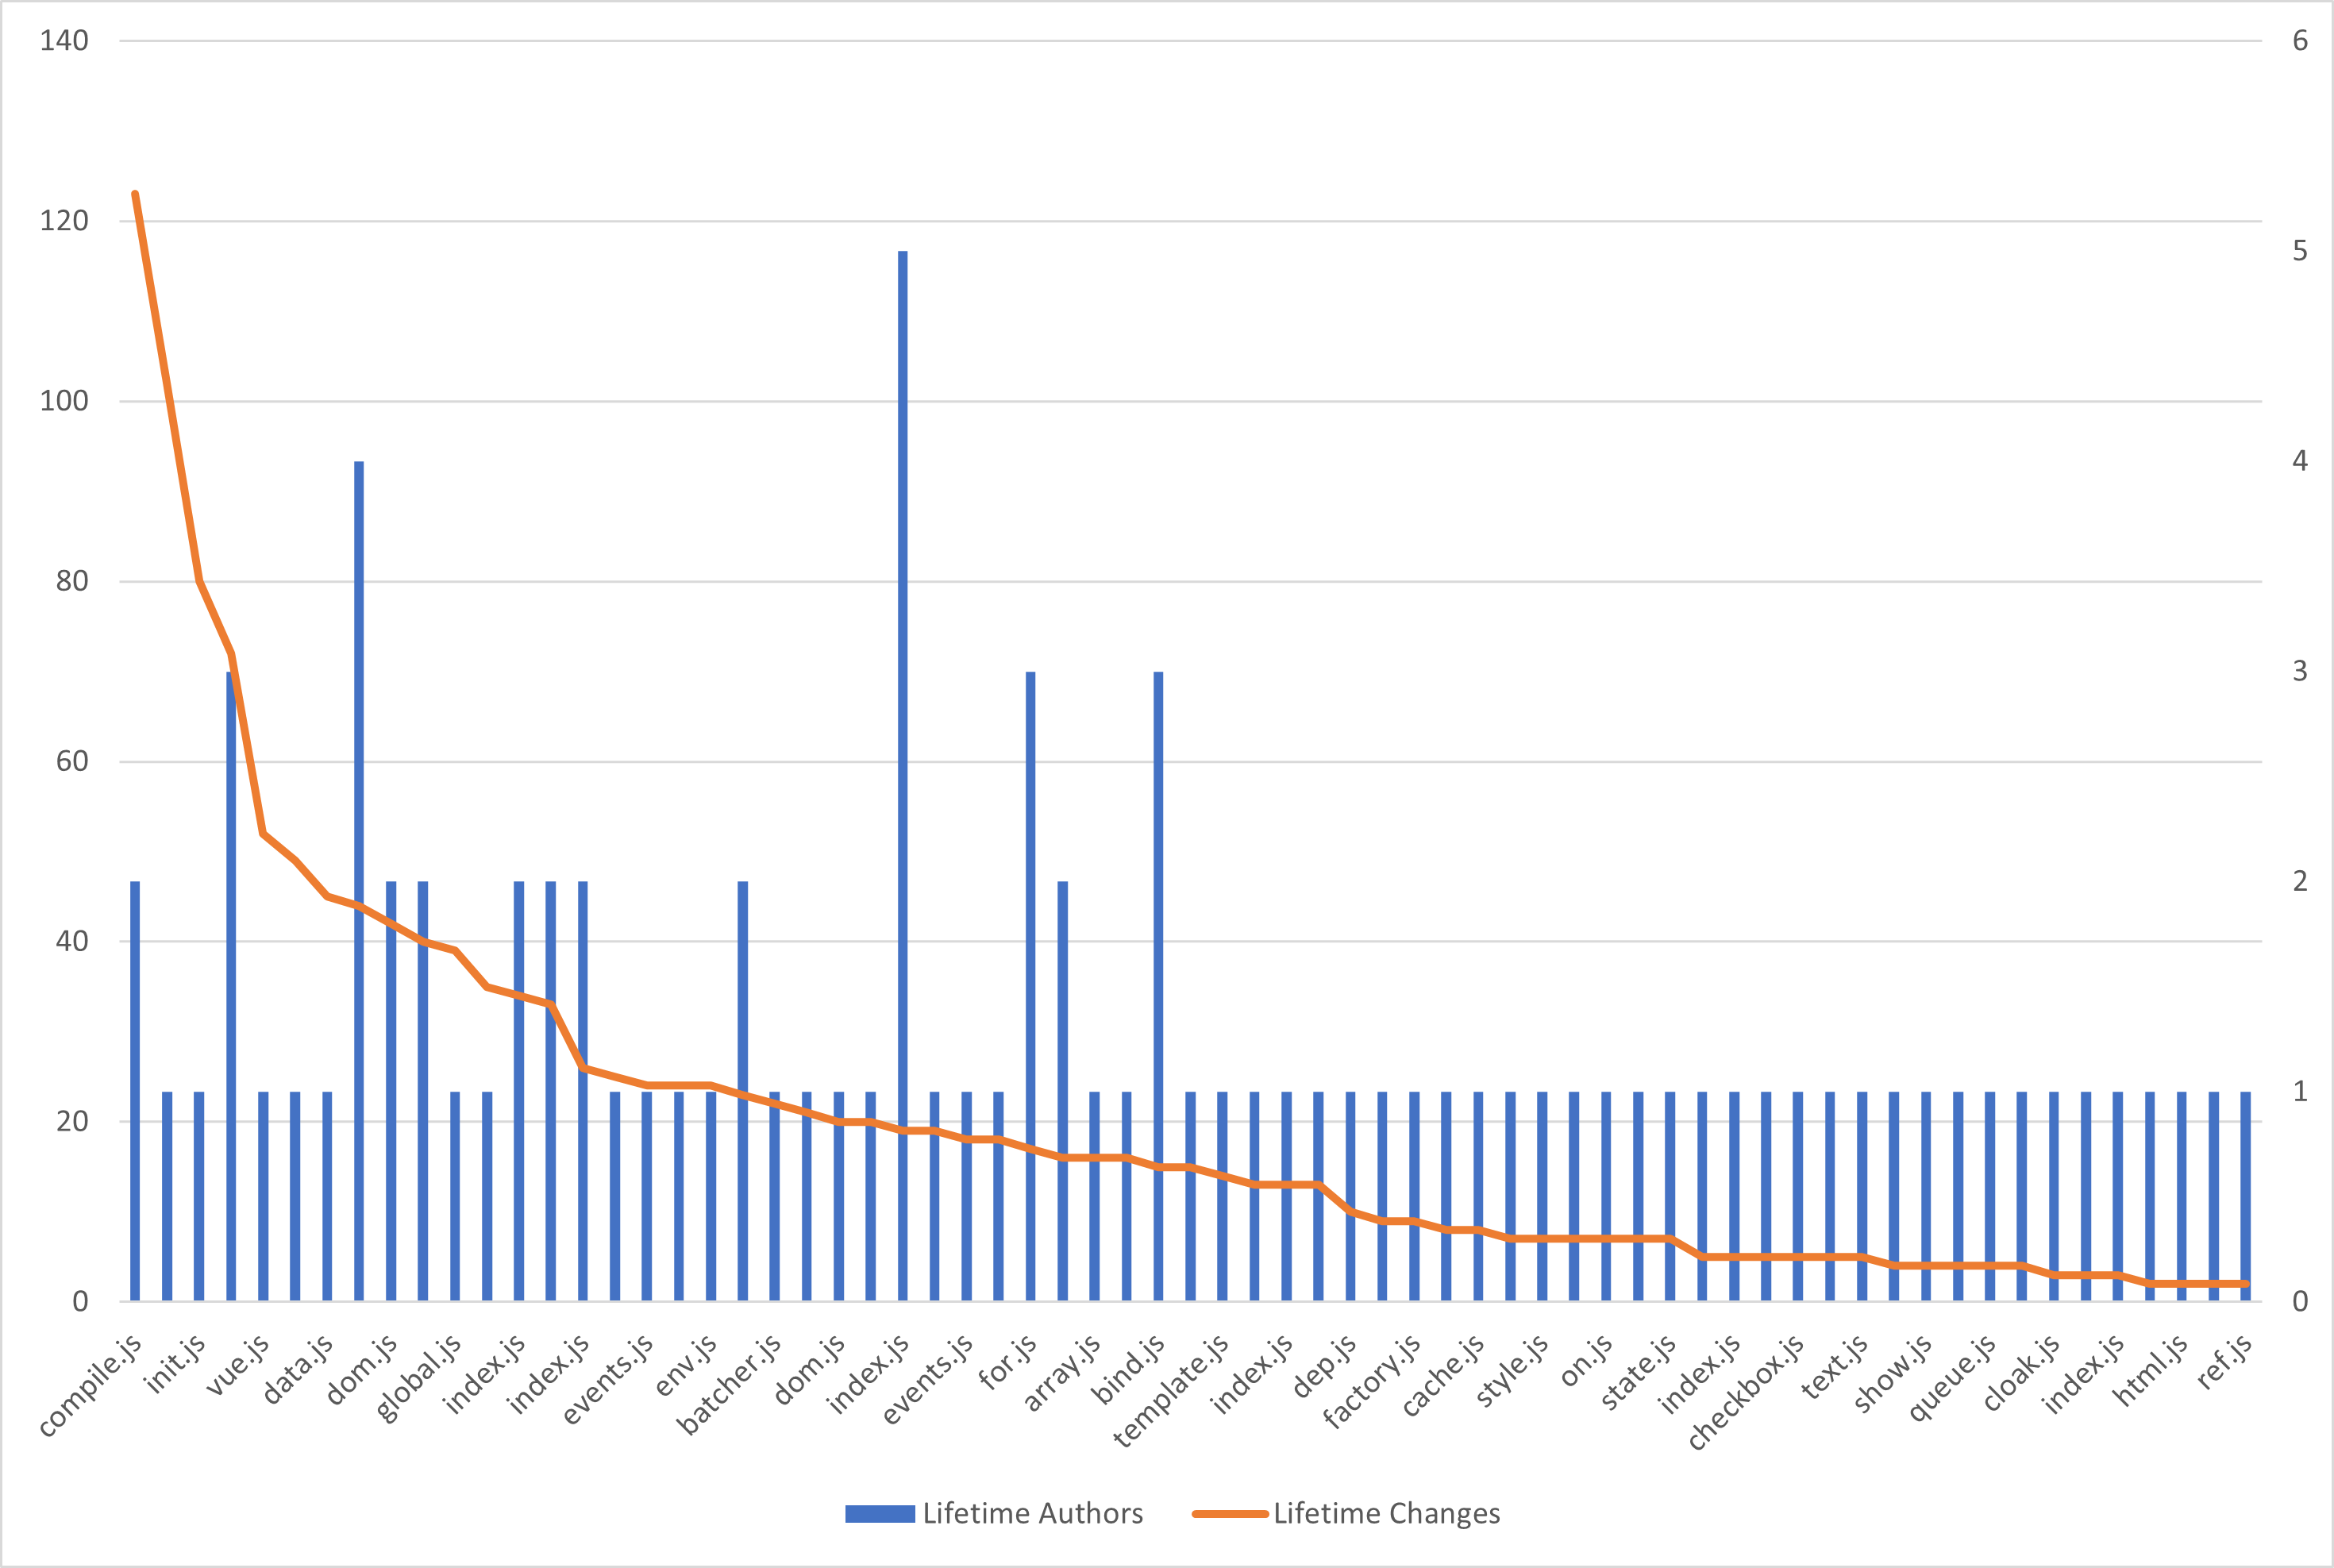
\includegraphics[width=1\textwidth]{images/vue/vue1-lifetimechanges-authors.png}
    \caption{A vékony kliens által generált grafikonok}
    \label{fig:hestia-charts}
\end{figure}

\begin{figure}[H]
    \centering
    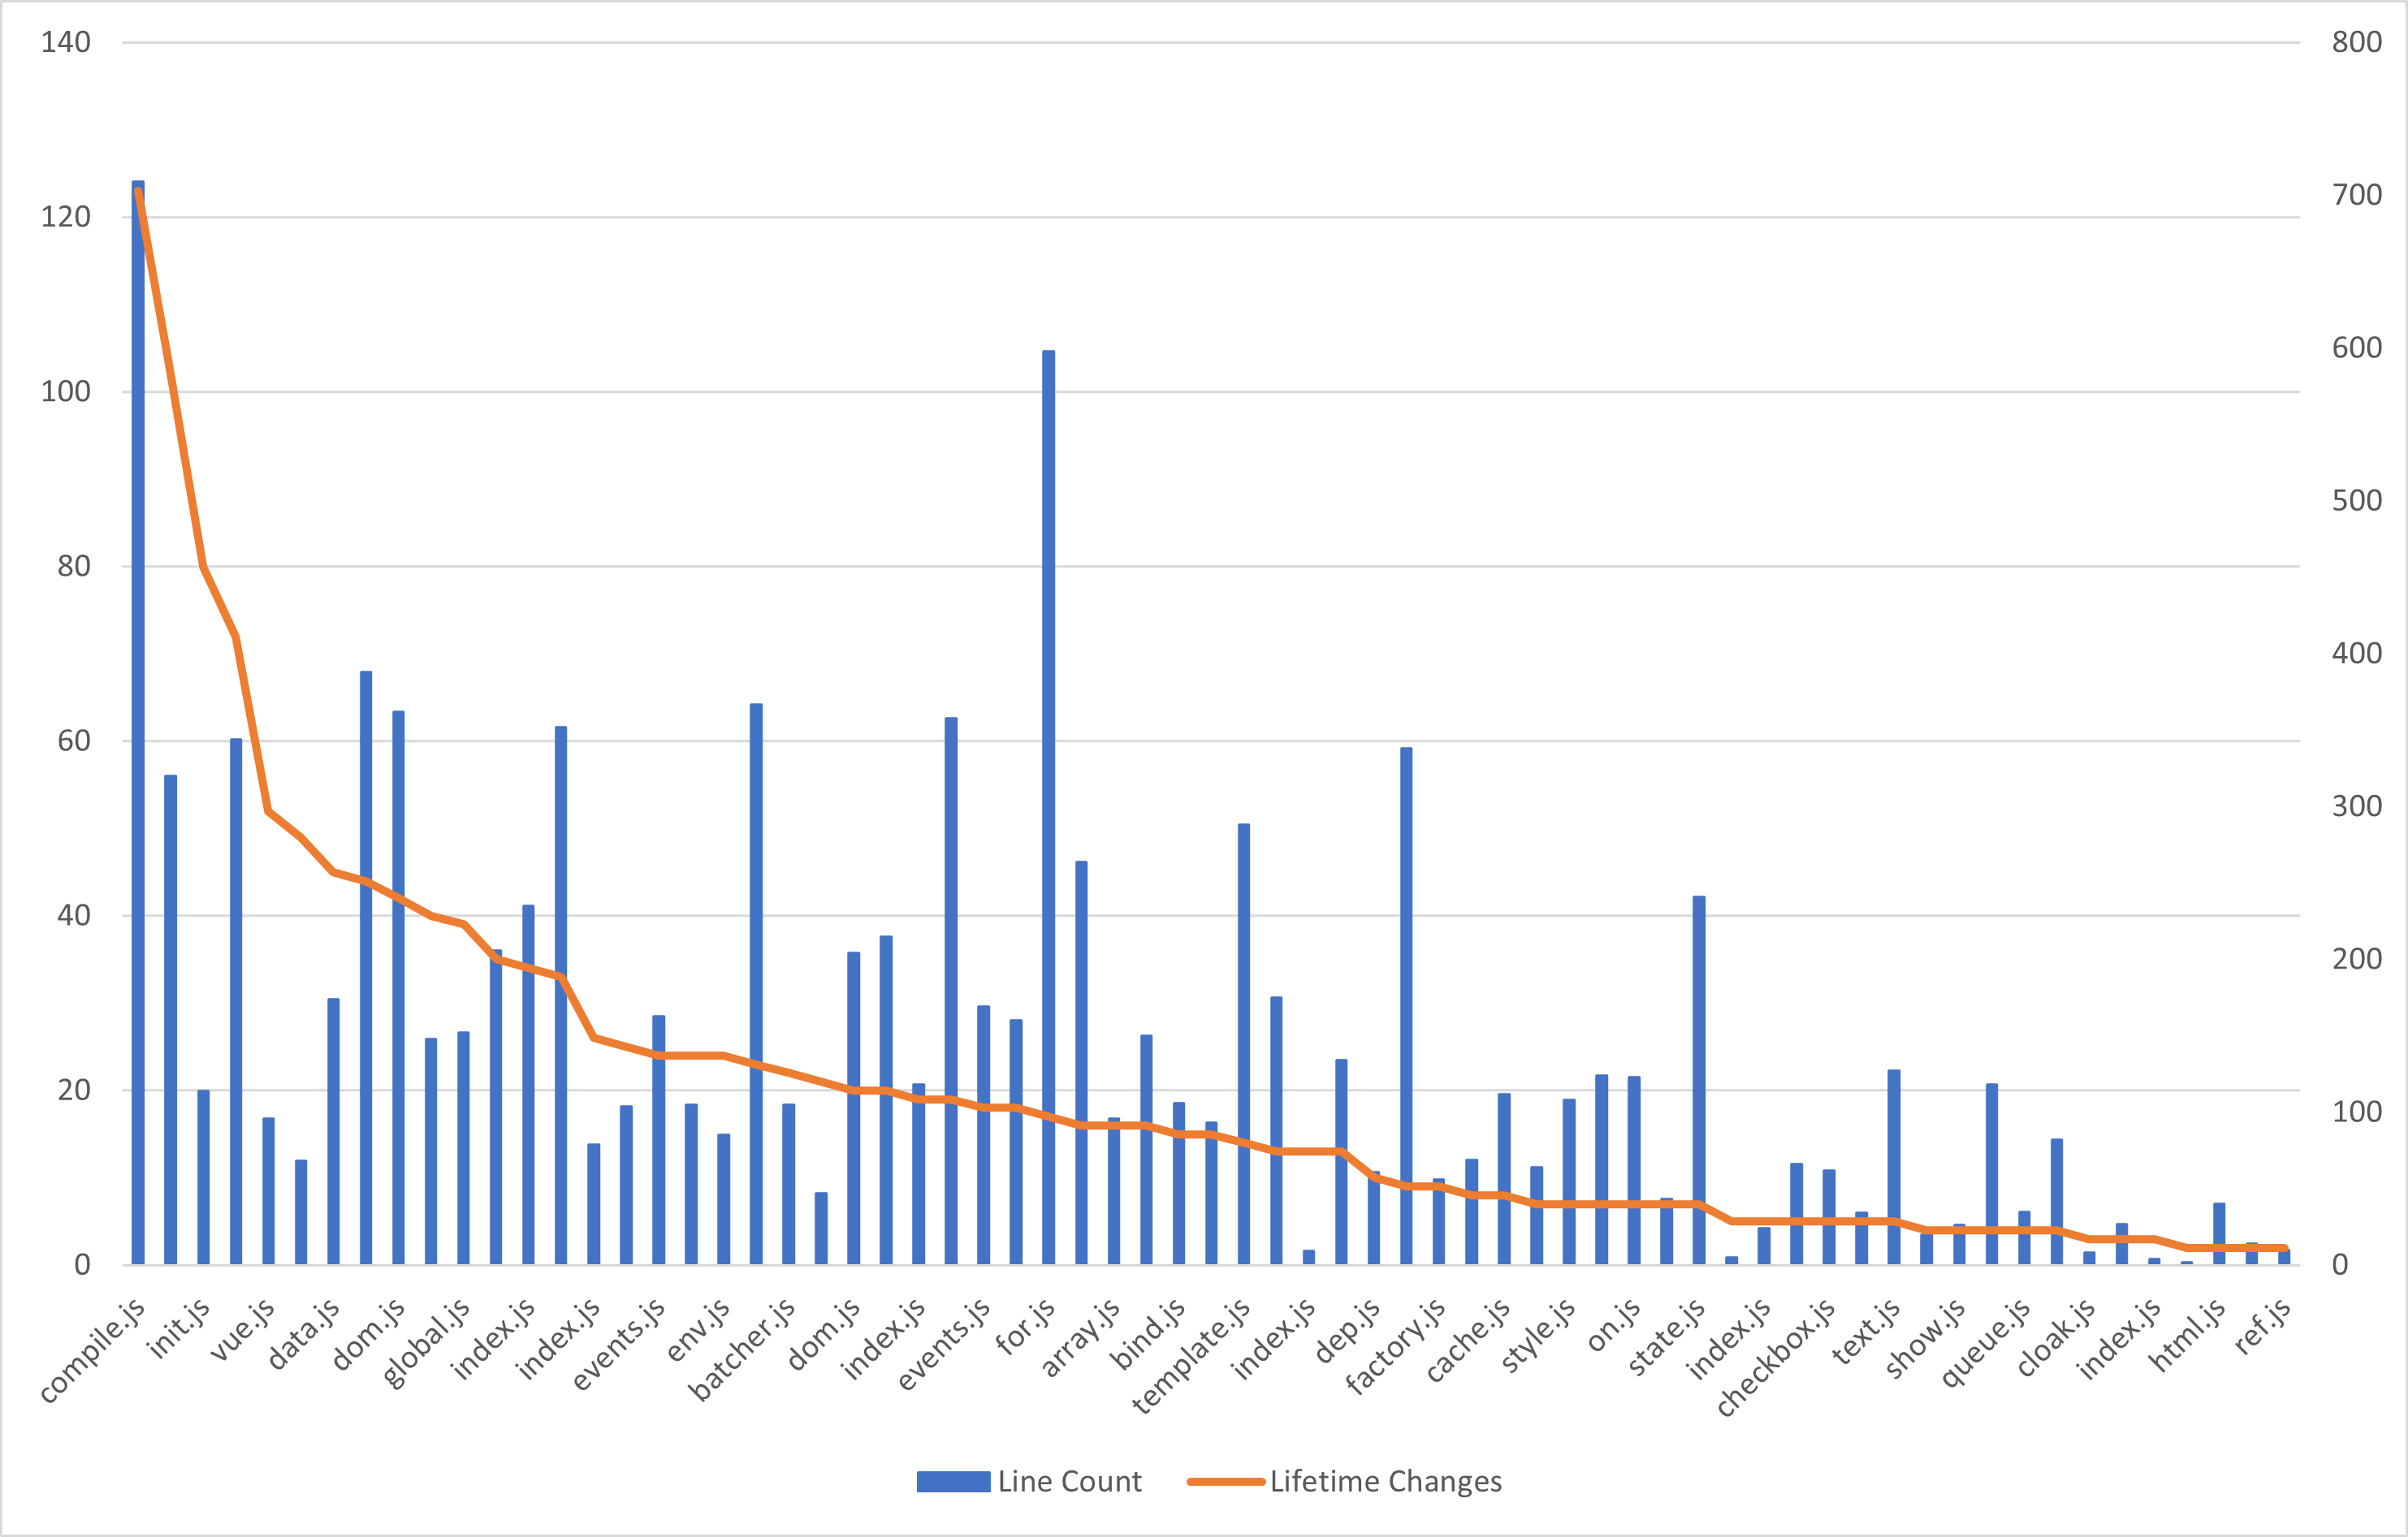
\includegraphics[width=1\textwidth]{images/vue/vue1-lines-lifetimechanges.png}
    \caption{A vékony kliens által generált grafikonok}
    \label{fig:hestia-charts}
\end{figure}

\pagebreak

\subsection{Vue 2.x}

\begin{table}[h]
    \hspace*{-1cm}\begin{tabular}{l|l|l|l|l}
        Filename                     & Lifetime Authors & Lifetime Changes & Line Count & Coverage \% \\ \hline
        compiler/parser/index.js     & 5                & 93               & 467        & 100         \\
        compiler/codegen/index.js    & 2                & 72               & 246        & 100         \\
        render.js                    & 2                & 67               & 253        & 100         \\
        create-component.js          & 4                & 56               & 296        & 100         \\
        patch.js                     & 2                & 54               & 524        & 100         \\
        transition.js                & 1                & 47               & 270        & 100         \\
        lifecycle.js                 & 3                & 45               & 201        & 100         \\
        helpers.js                   & 2                & 34               & 145        & 100         \\
        web-runtime-with-compiler.js & 3                & 33               & 84         & 100         \\
        core/index.js                & 1                & 31               & 13         & 100
    \end{tabular}
    \caption{A vue 1.0-ás kiadásának leggyakrabban módosított fájljai} \label{table:vue2-top-files}
\end{table}

\begin{figure}[H]
    \centering
    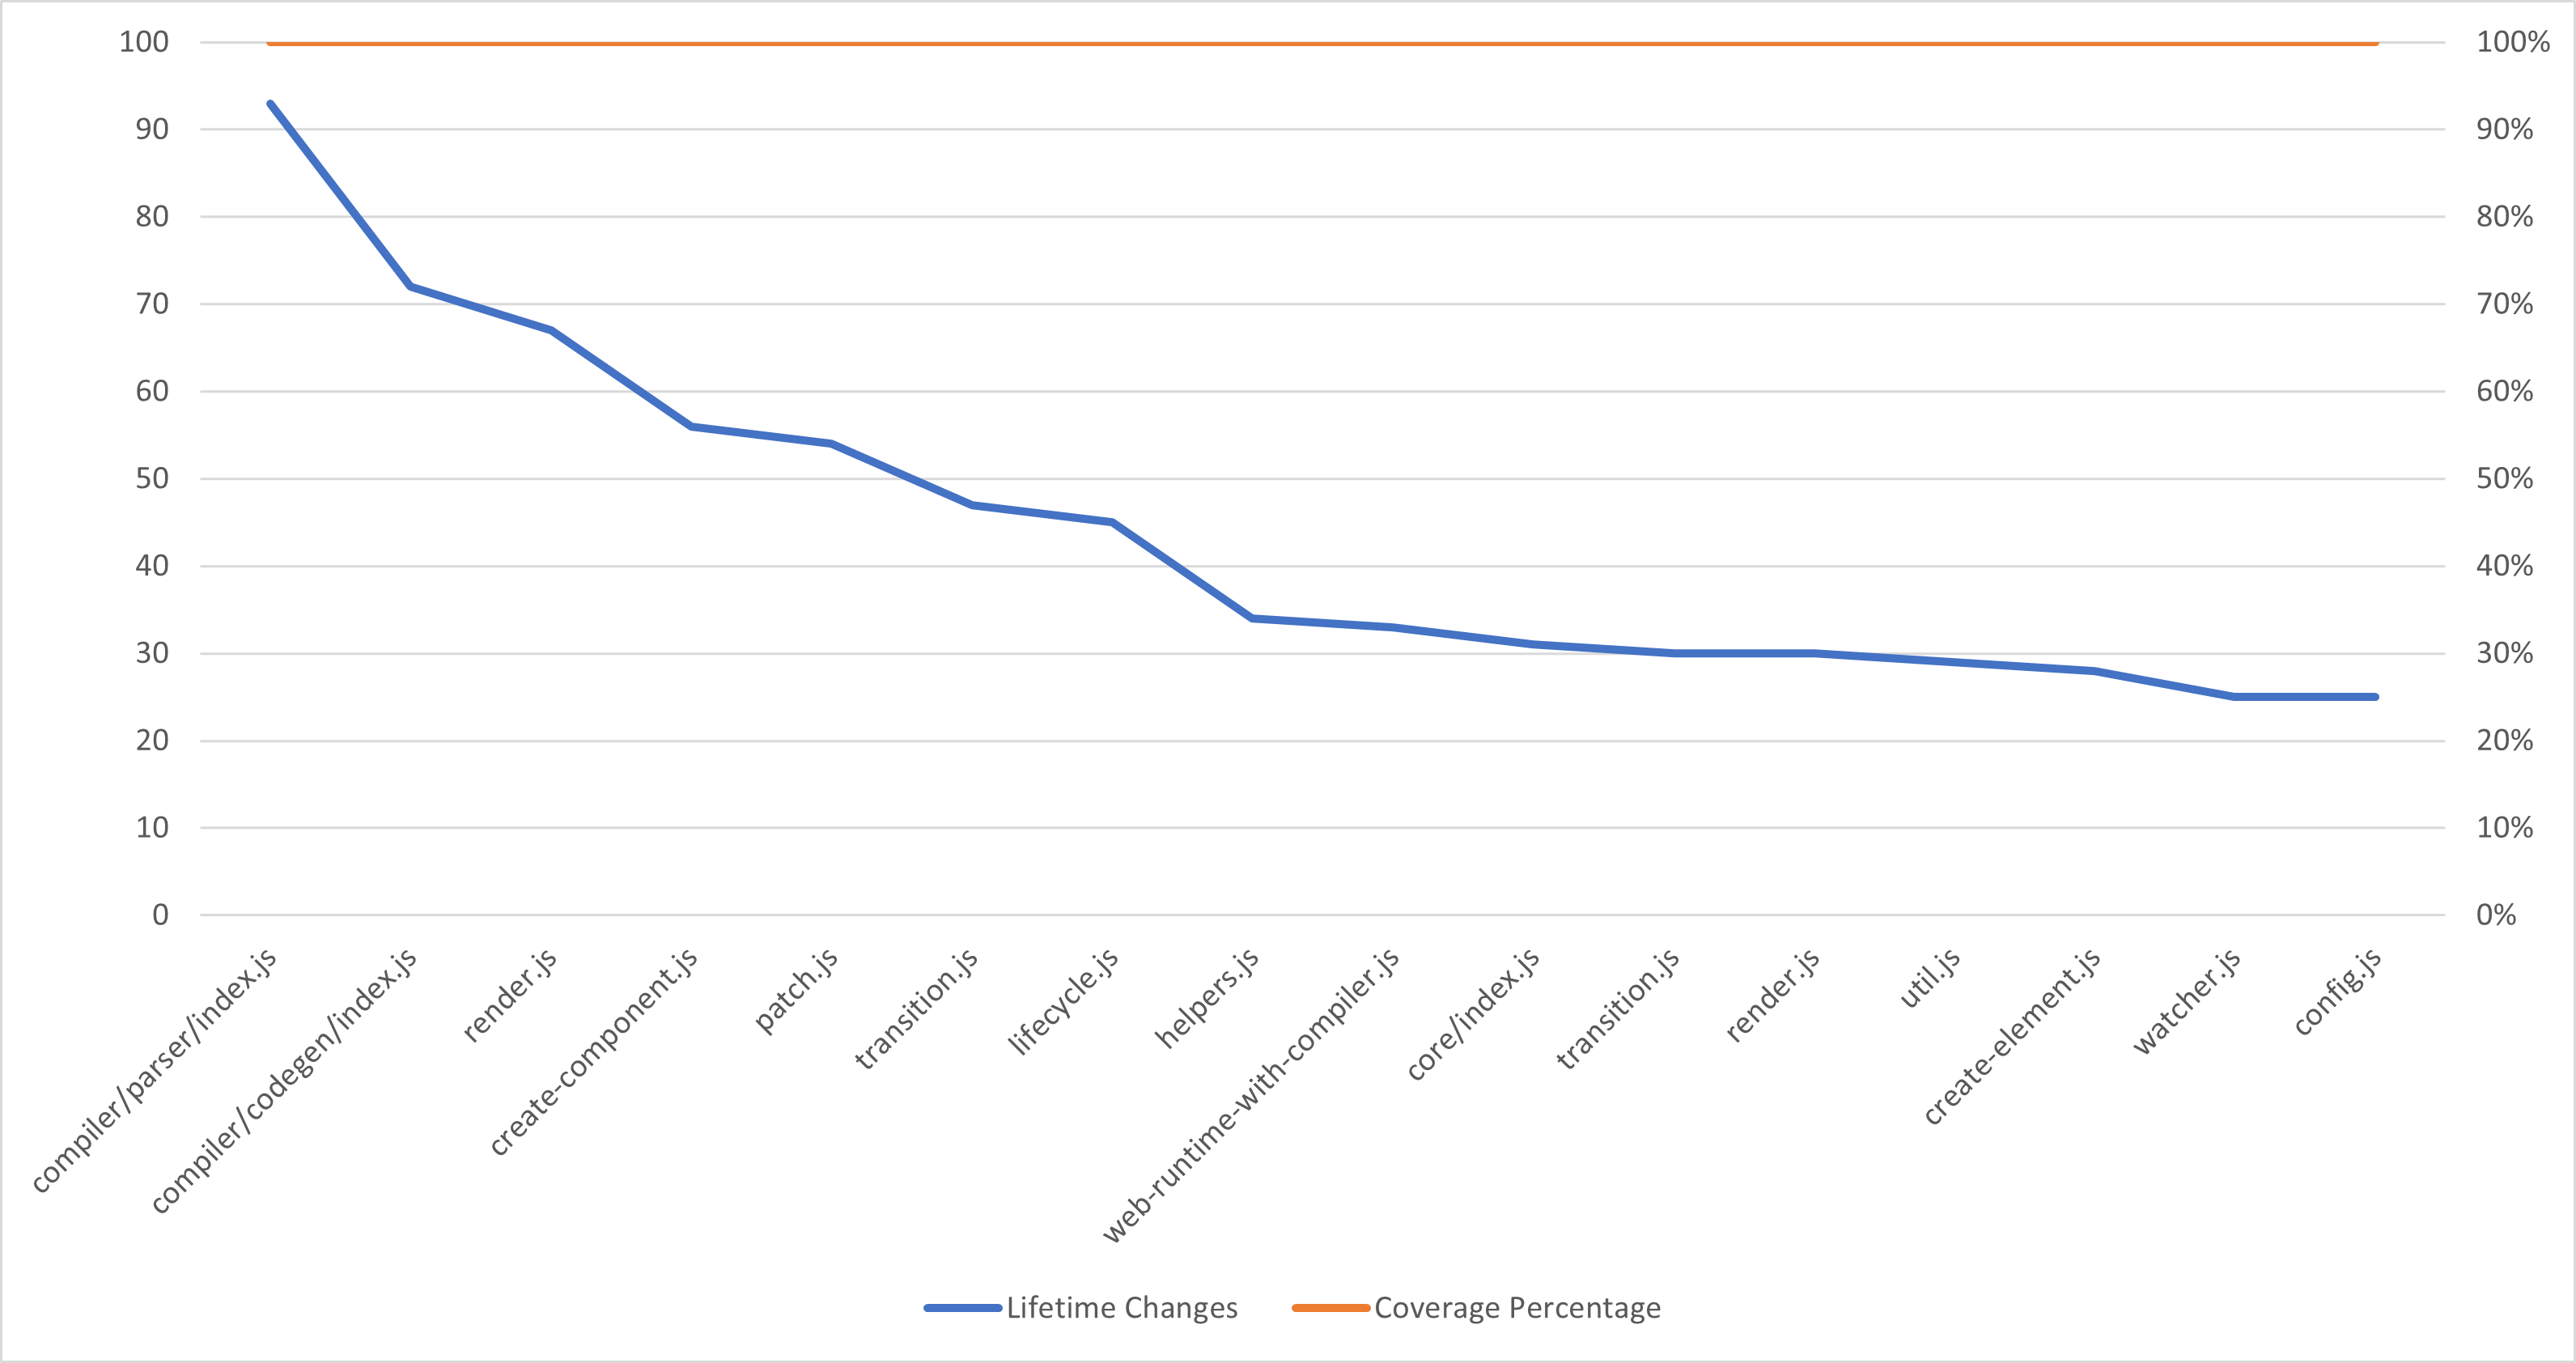
\includegraphics[width=1\textwidth]{images/vue/vue2-lifetime-changes.png}
    \caption{A vékony kliens által generált grafikonok}
    \label{fig:hestia-charts}
\end{figure}

\begin{figure}[H]
    \centering
    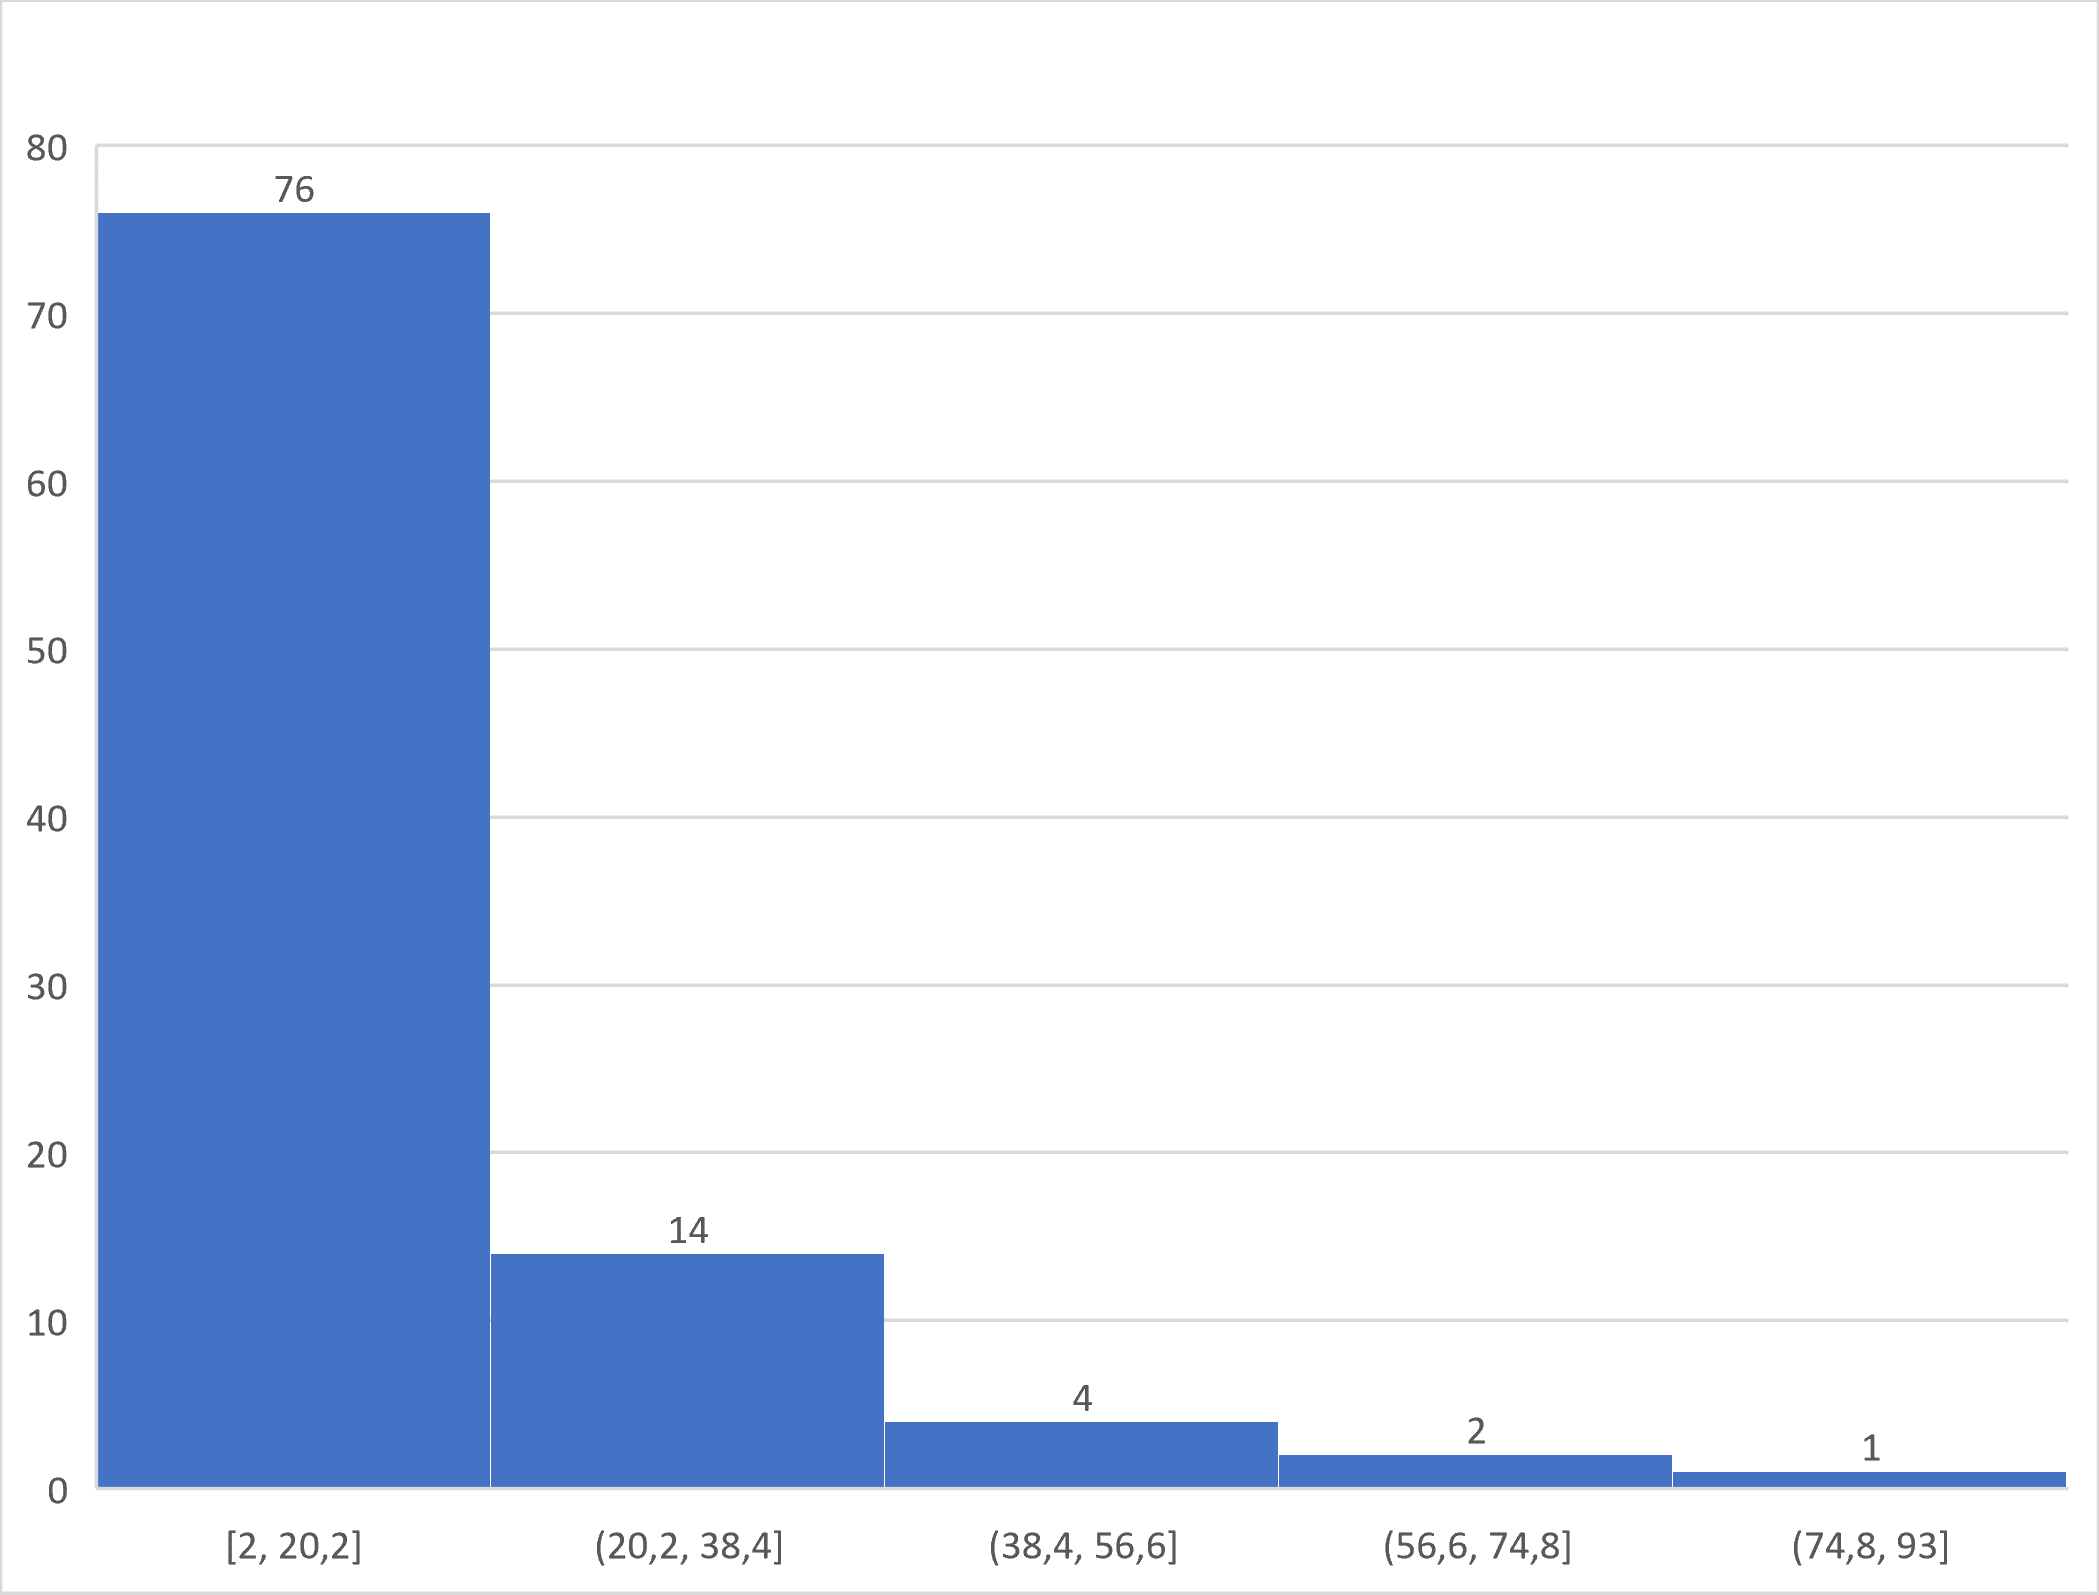
\includegraphics[width=1\textwidth]{images/vue/vue2-hist.png}
    \caption{A vékony kliens által generált grafikonok}
    \label{fig:hestia-charts}
\end{figure}

\begin{figure}[H]
    \centering
    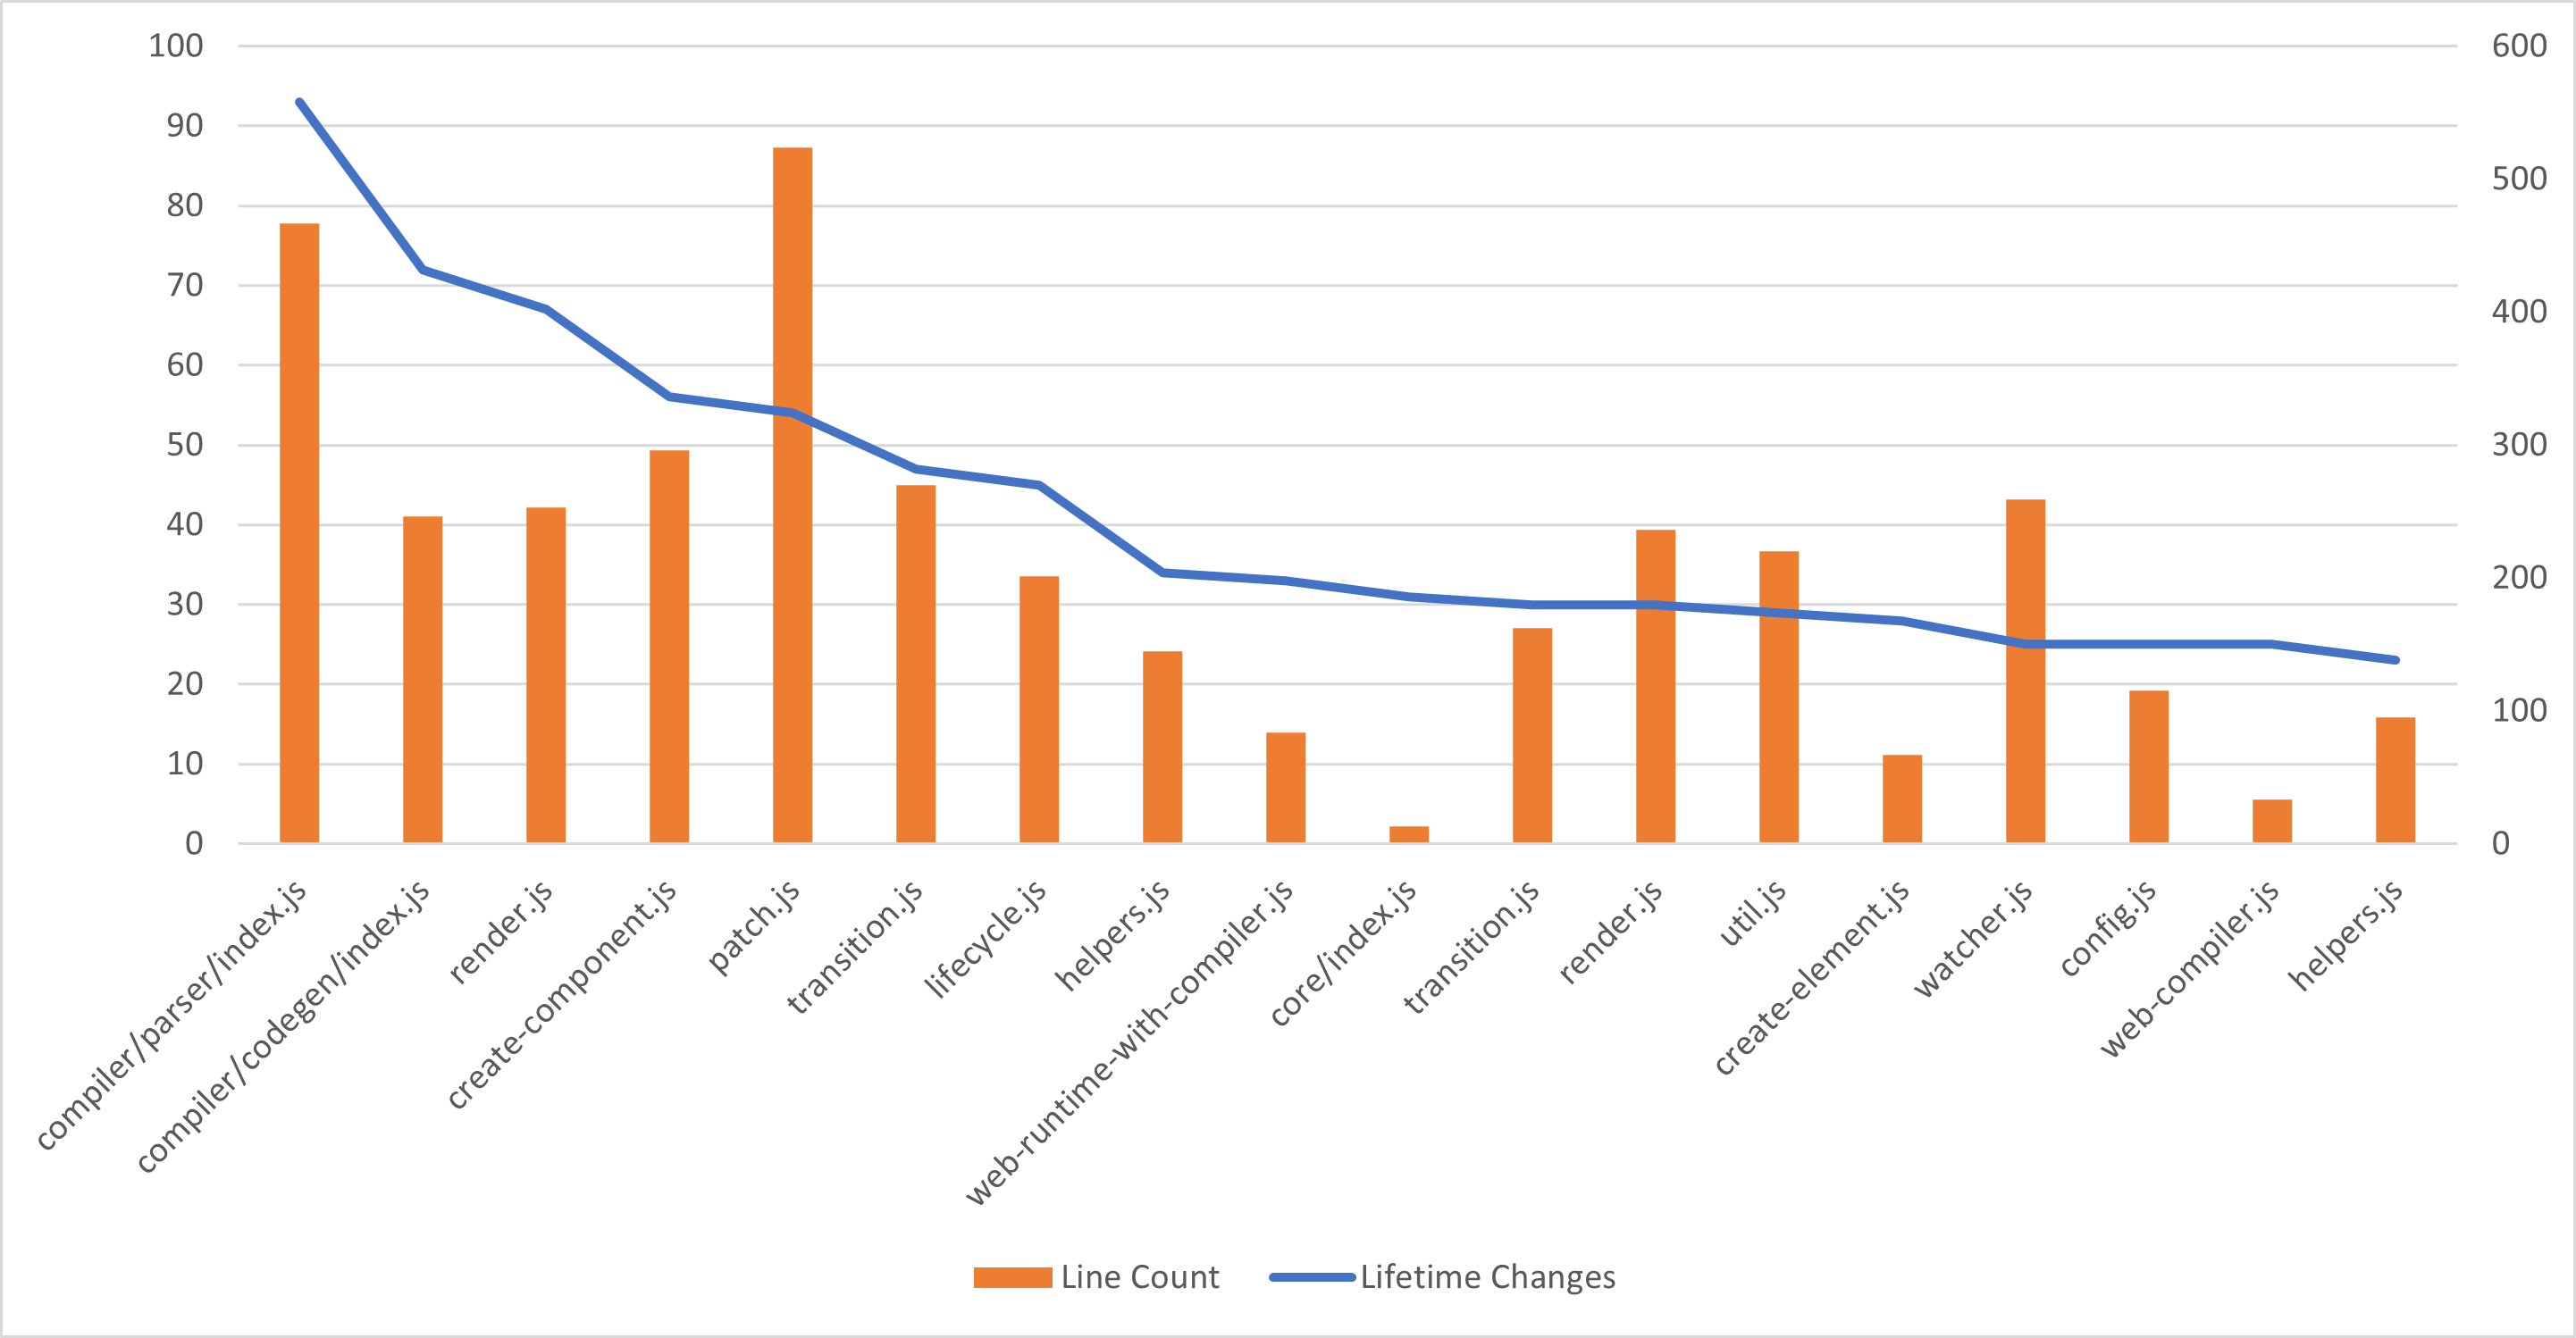
\includegraphics[width=1\textwidth]{images/vue/vue2-lines-lifetimechanges.png}
    \caption{A vékony kliens által generált grafikonok}
    \label{fig:hestia-charts}
\end{figure}

\subsubsection{Átfedések vue 1.x és 2.0 között}

\begin{figure}[H]
    \centering
    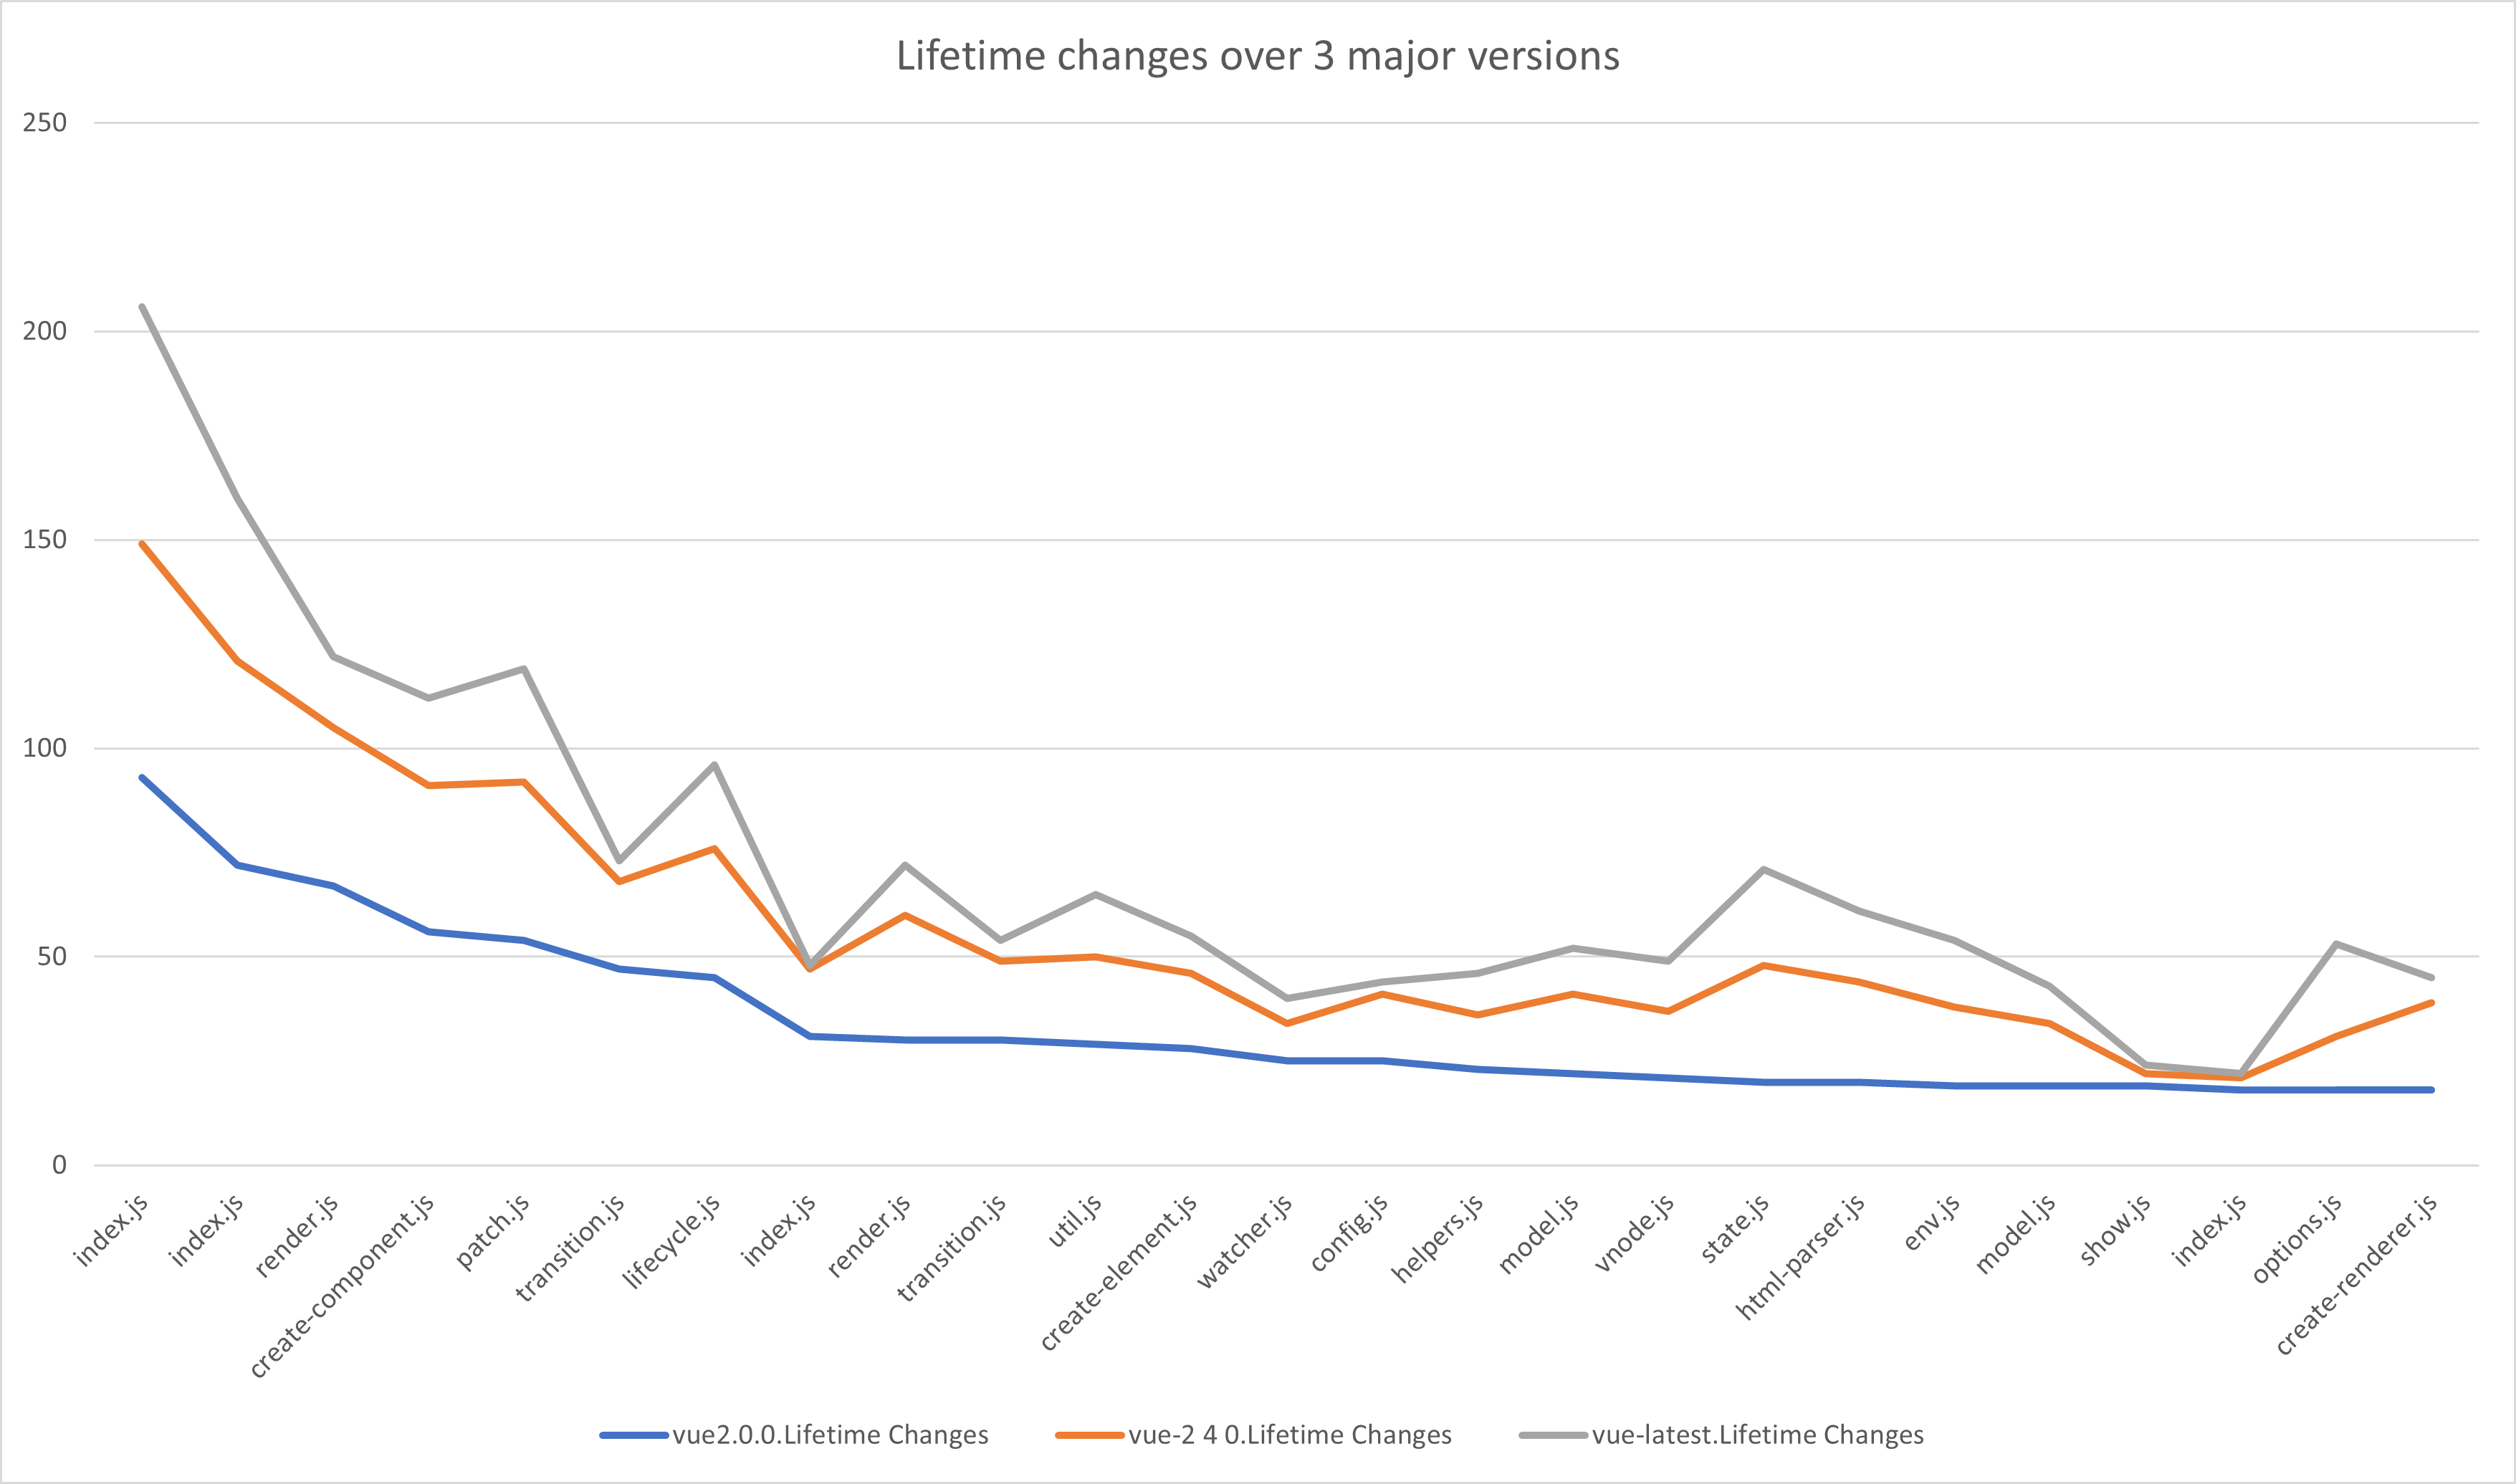
\includegraphics[width=1\textwidth]{images/vue/vue-all-lifetime-changes.png}
    \caption{A vékony kliens által generált grafikonok}
    \label{fig:hestia-charts}
\end{figure}

\begin{figure}[H]
    \centering
    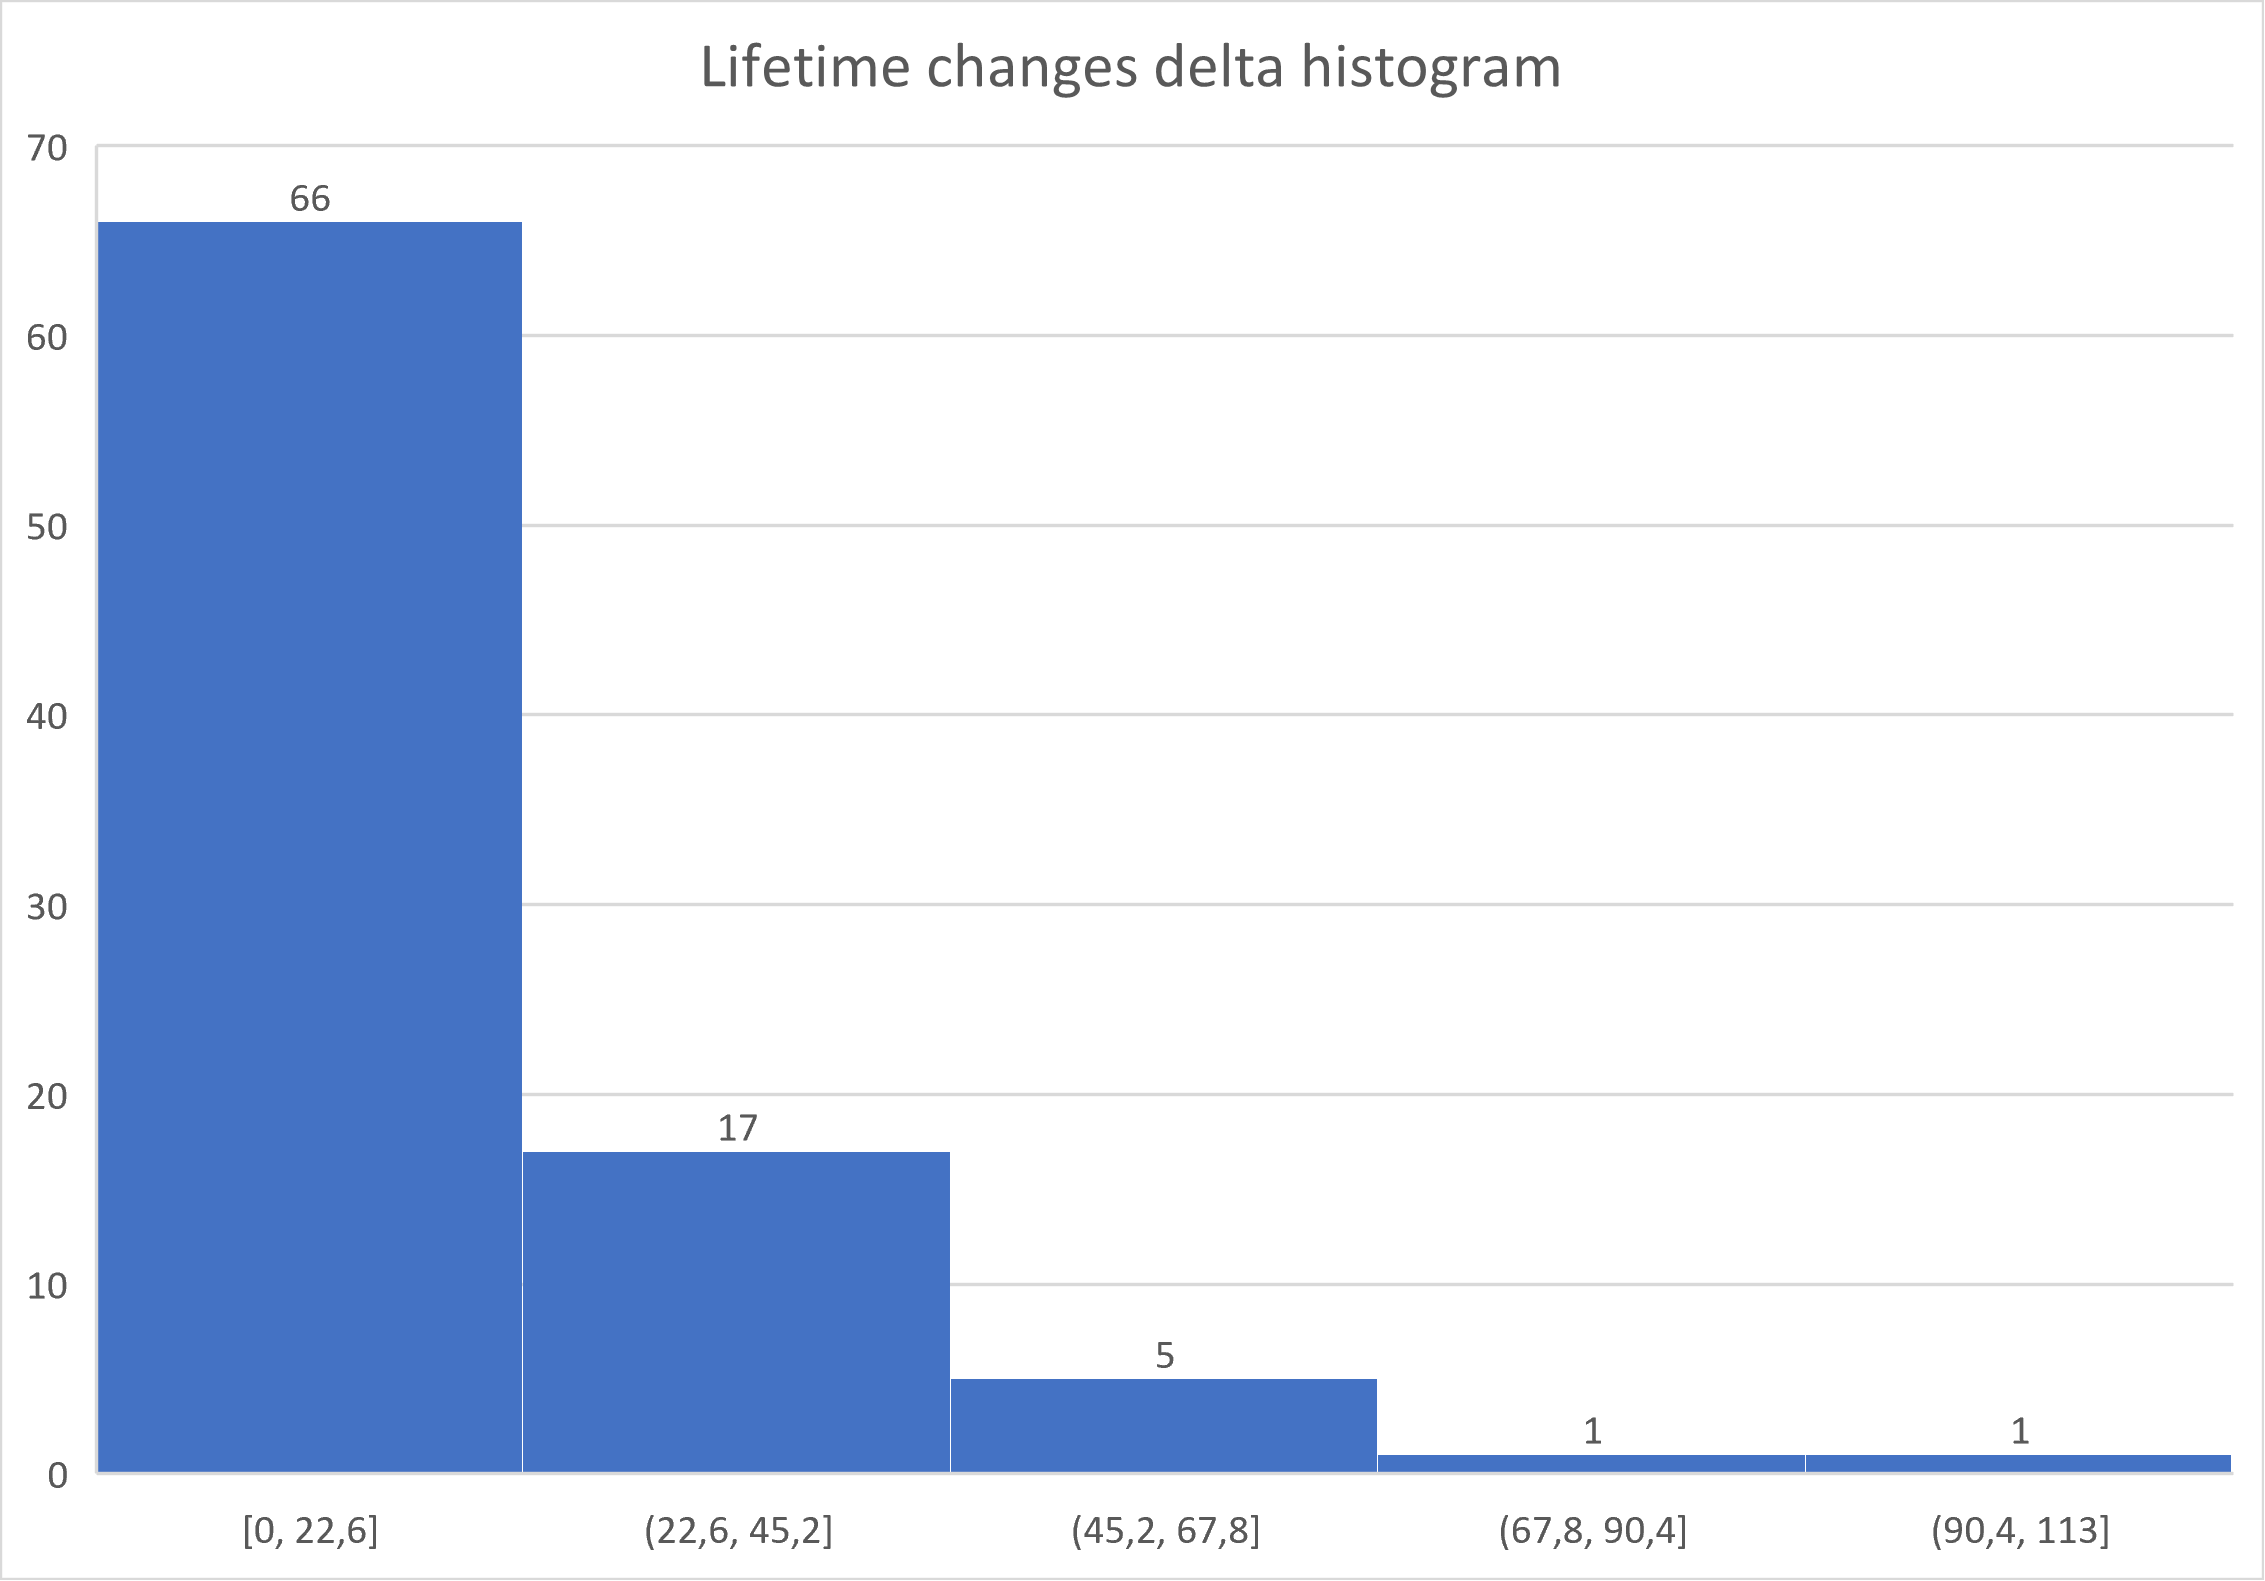
\includegraphics[width=1\textwidth]{images/vue/vue-all-lifetime-changes-delta-hist.png}
    \caption{A vékony kliens által generált grafikonok}
    \label{fig:hestia-charts}
\end{figure}

\begin{figure}[H]
    \centering
    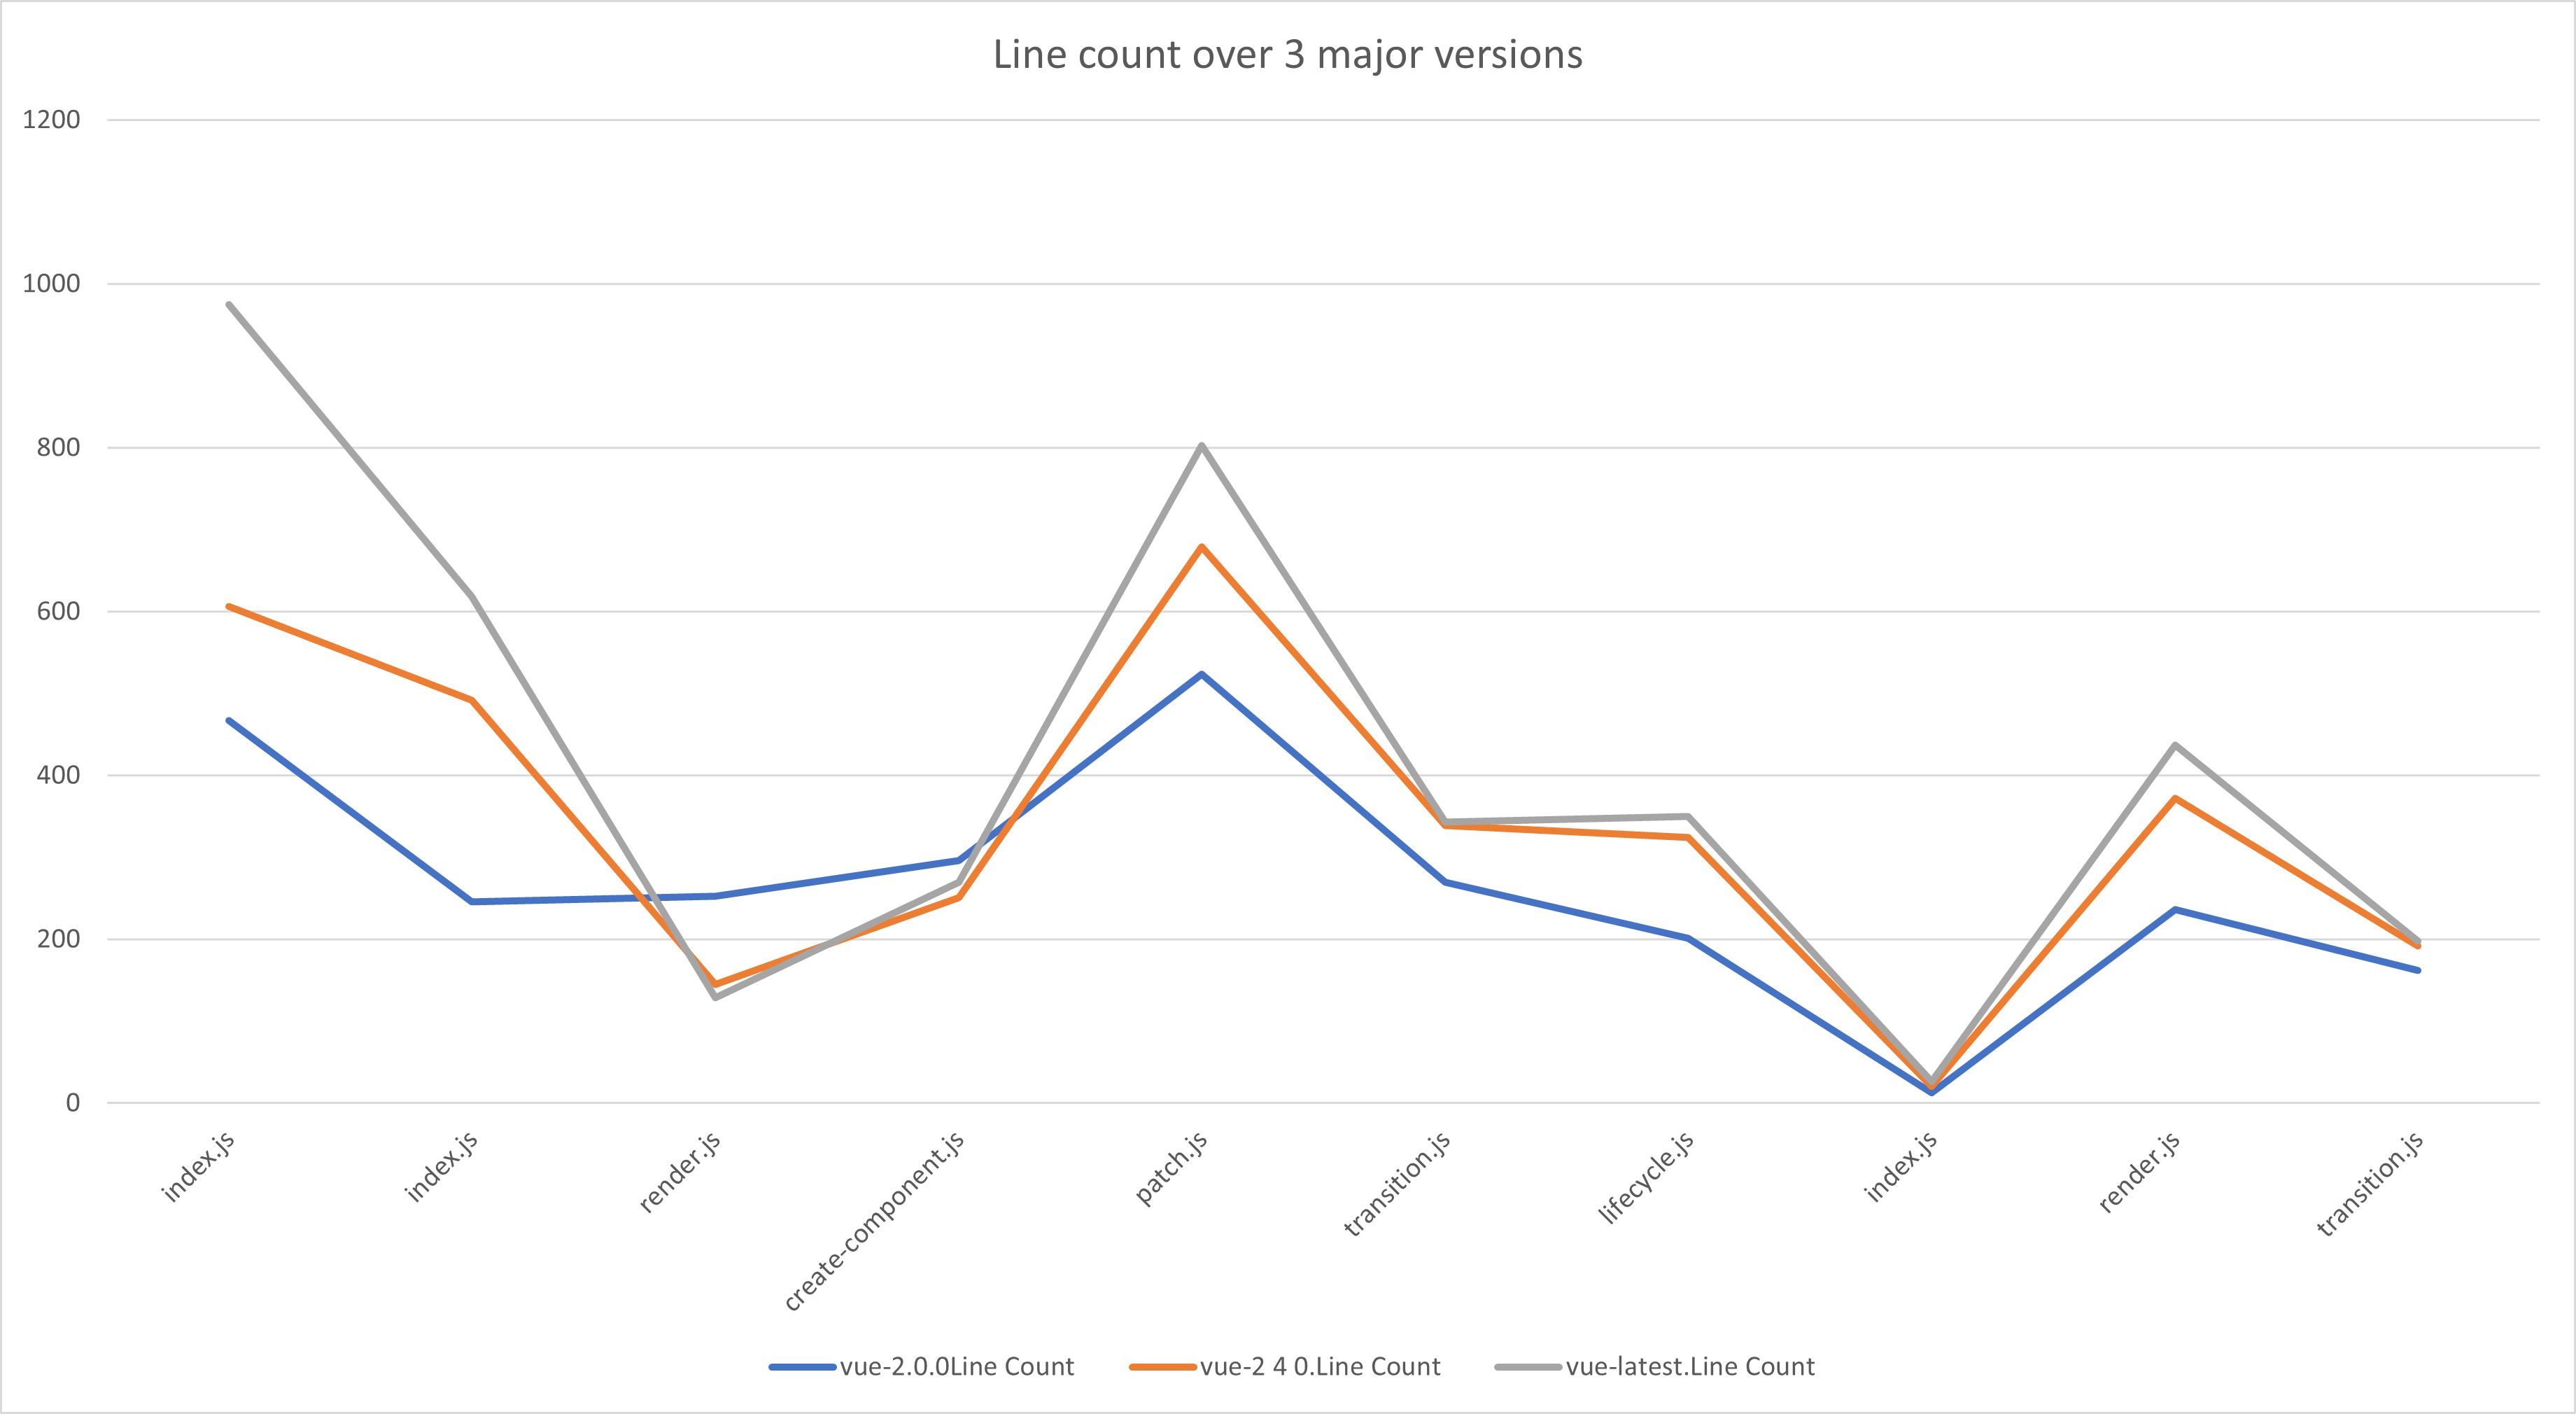
\includegraphics[width=1\textwidth]{images/vue/vue-all-line-count.png}
    \caption{A vékony kliens által generált grafikonok}
    \label{fig:hestia-charts}
\end{figure}

\begin{figure}[H]
    \centering
    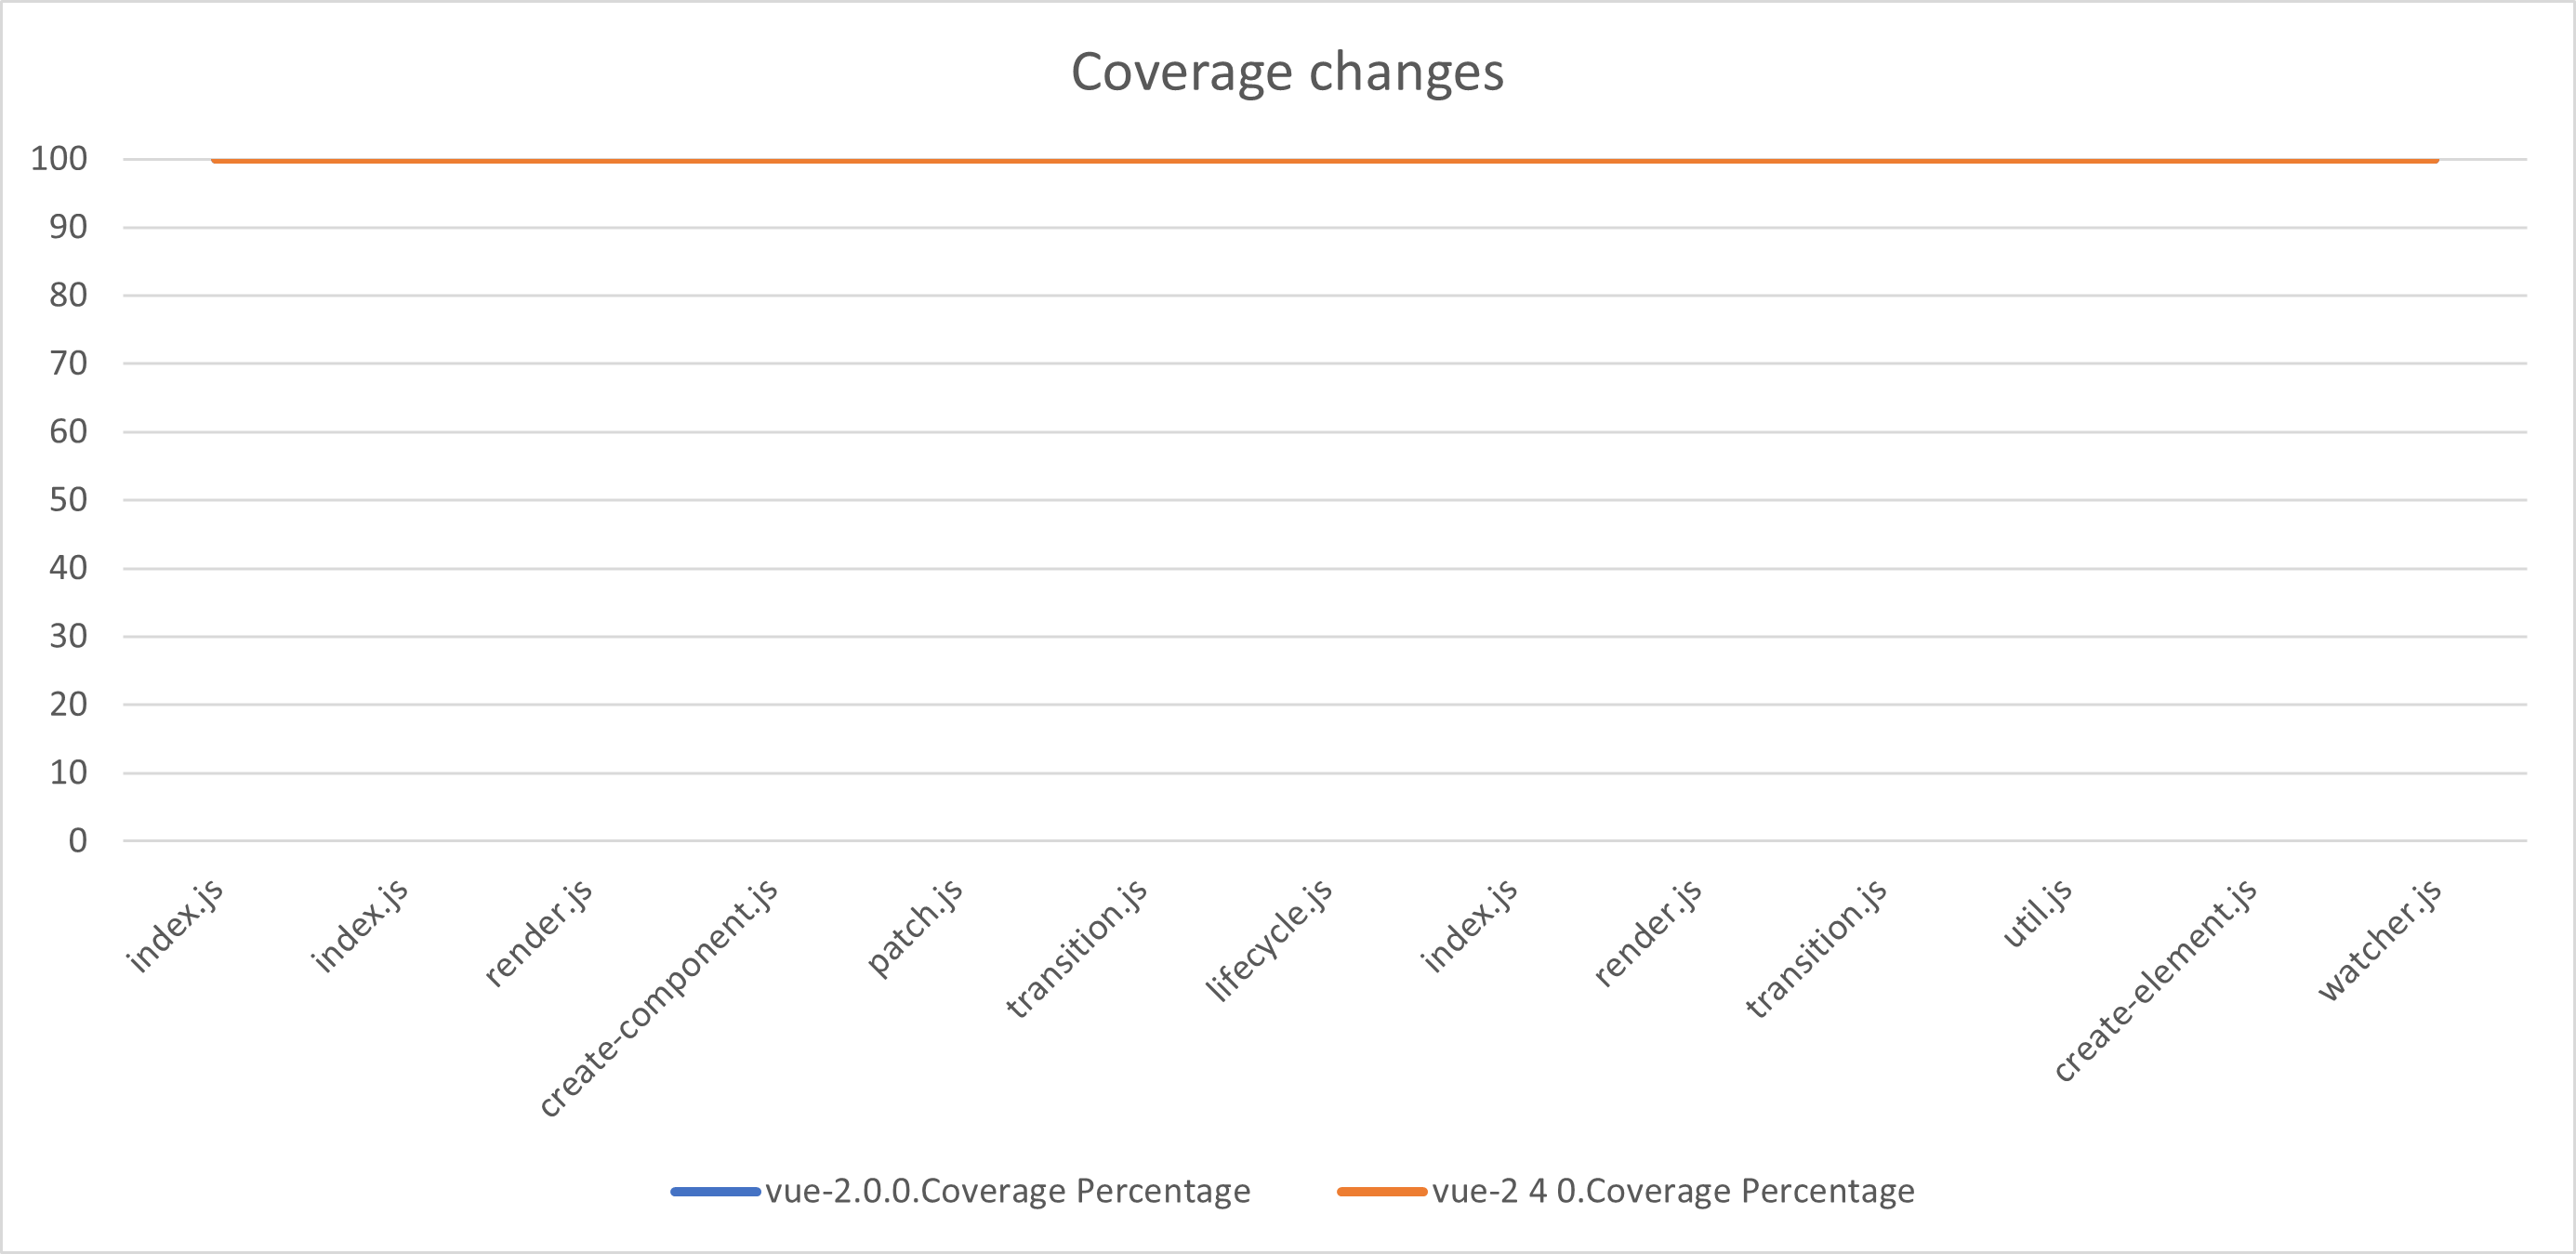
\includegraphics[width=1\textwidth]{images/vue/vue-all-coverage.png}
    \caption{A vékony kliens által generált grafikonok}
    \label{fig:hestia-charts}
\end{figure}

\begin{table}[]
    \centering
    \begin{tabular}{l|l|l|l}
                                          & v2.0.0 & v2.4.0 & dev  \\ \hline
        Total no of commits               & 1147   & 1692   & 2082 \\
        Sum of commits top 10 involved in & 525    & 858    & 1062
    \end{tabular}
    \caption{}\label{tab:my-table}
\end{table}

\section{React}

\section{Moment.js}

\section{Összehasonlítás}